\documentclass[twoside]{book}

% Packages required by doxygen
\usepackage{calc}
\usepackage{doxygen}
\usepackage{graphicx}
\usepackage[utf8]{inputenc}
\usepackage{makeidx}
\usepackage{multicol}
\usepackage{multirow}
\usepackage{textcomp}
\usepackage[table]{xcolor}

% Font selection
\usepackage[T1]{fontenc}
\usepackage{mathptmx}
\usepackage[scaled=.90]{helvet}
\usepackage{courier}
\usepackage{amssymb}
\usepackage{sectsty}
\renewcommand{\familydefault}{\sfdefault}
\allsectionsfont{%
  \fontseries{bc}\selectfont%
  \color{darkgray}%
}
\renewcommand{\DoxyLabelFont}{%
  \fontseries{bc}\selectfont%
  \color{darkgray}%
}

% Page & text layout
\usepackage{geometry}
\geometry{%
  a4paper,%
  top=2.5cm,%
  bottom=2.5cm,%
  left=2.5cm,%
  right=2.5cm%
}
\tolerance=750
\hfuzz=15pt
\hbadness=750
\setlength{\emergencystretch}{15pt}
\setlength{\parindent}{0cm}
\setlength{\parskip}{0.2cm}
\makeatletter
\renewcommand{\paragraph}{%
  \@startsection{paragraph}{4}{0ex}{-1.0ex}{1.0ex}{%
    \normalfont\normalsize\bfseries\SS@parafont%
  }%
}
\renewcommand{\subparagraph}{%
  \@startsection{subparagraph}{5}{0ex}{-1.0ex}{1.0ex}{%
    \normalfont\normalsize\bfseries\SS@subparafont%
  }%
}
\makeatother

% Headers & footers
\usepackage{fancyhdr}
\pagestyle{fancyplain}
\fancyhead[LE]{\fancyplain{}{\bfseries\thepage}}
\fancyhead[CE]{\fancyplain{}{}}
\fancyhead[RE]{\fancyplain{}{\bfseries\leftmark}}
\fancyhead[LO]{\fancyplain{}{\bfseries\rightmark}}
\fancyhead[CO]{\fancyplain{}{}}
\fancyhead[RO]{\fancyplain{}{\bfseries\thepage}}
\fancyfoot[LE]{\fancyplain{}{}}
\fancyfoot[CE]{\fancyplain{}{}}
\fancyfoot[RE]{\fancyplain{}{\bfseries\scriptsize Generated on Mon May 16 2016 15\-:54\-:02 for Skye\-Controls by Doxygen }}
\fancyfoot[LO]{\fancyplain{}{\bfseries\scriptsize Generated on Mon May 16 2016 15\-:54\-:02 for Skye\-Controls by Doxygen }}
\fancyfoot[CO]{\fancyplain{}{}}
\fancyfoot[RO]{\fancyplain{}{}}
\renewcommand{\footrulewidth}{0.4pt}
\renewcommand{\chaptermark}[1]{%
  \markboth{#1}{}%
}
\renewcommand{\sectionmark}[1]{%
  \markright{\thesection\ #1}%
}

% Indices & bibliography
\usepackage{natbib}
\usepackage[titles]{tocloft}
\setcounter{tocdepth}{3}
\setcounter{secnumdepth}{5}
\makeindex

% Hyperlinks (required, but should be loaded last)
\usepackage{ifpdf}
\ifpdf
  \usepackage[pdftex,pagebackref=true]{hyperref}
\else
  \usepackage[ps2pdf,pagebackref=true]{hyperref}
\fi
\hypersetup{%
  colorlinks=true,%
  linkcolor=blue,%
  citecolor=blue,%
  unicode%
}

% Custom commands
\newcommand{\clearemptydoublepage}{%
  \newpage{\pagestyle{empty}\cleardoublepage}%
}


%===== C O N T E N T S =====

\begin{document}

% Titlepage & ToC
\hypersetup{pageanchor=false}
\pagenumbering{roman}
\begin{titlepage}
\vspace*{7cm}
\begin{center}%
{\Large Skye\-Controls \\[1ex]\large 1.\-00 }\\
\vspace*{1cm}
{\large Generated by Doxygen 1.8.6}\\
\vspace*{0.5cm}
{\small Mon May 16 2016 15:54:02}\\
\end{center}
\end{titlepage}
\clearemptydoublepage
\tableofcontents
\clearemptydoublepage
\pagenumbering{arabic}
\hypersetup{pageanchor=true}

%--- Begin generated contents ---
\chapter{Simulation Framework For Skye}
\label{md__r_e_a_d_m_e}
\hypertarget{md__r_e_a_d_m_e}{}
This repository contains everything you need to simulate the airship Skye in \href{http://gazebosim.org/}{\tt Gazebo} and interact with it by using the Robotic Operating System \href{http://www.ros.org/}{\tt R\-O\-S}. The recommended O\-S is Ubuntu 14.\-04.

\subsection*{R\-O\-S Installation}

These steps are taken from the main installation page of R\-O\-S. Configure your Ubuntu repositories to allow \char`\"{}restricted,\char`\"{} \char`\"{}universe,\char`\"{} and \char`\"{}multiverse.\char`\"{} You can \href{https://help.ubuntu.com/community/Repositories/Ubuntu}{\tt follow the Ubuntu guide} for instructions on doing this. Setup your computer to accept software from packages.\-ros.\-org. R\-O\-S Indigo O\-N\-L\-Y supports Saucy (13.\-10) and Trusty (14.\-04) for debian packages. ```bash sudo sh -\/c 'echo \char`\"{}deb http\-://packages.\-ros.\-org/ros/ubuntu \$(lsb\-\_\-release -\/sc) main\char`\"{} $>$ /etc/apt/sources.list.\-d/ros-\/latest.list' ``` Set up your keys ```bash sudo apt-\/key adv --keyserver hkp\-://ha.pool.\-sks-\/keyservers.\-net --recv-\/key 0x\-B01\-F\-A116 ``` Installation\-: first, make sure your Debian package index is up-\/to-\/date. ```bash sudo apt-\/get update ``` Install the Desktop Install version, which provides you\-: R\-O\-S, rqt, rviz, and robot-\/generic libraries ```bash sudo apt-\/get install ros-\/indigo-\/desktop ``` Initialize R\-O\-S. ```bash sudo rosdep init rosdep update ``` It's convenient if the R\-O\-S environment variables are automatically added to your bash session every time a new shell is launched\-: ```bash echo \char`\"{}source /opt/ros/indigo/setup.\-bash\char`\"{} $>$$>$ $\sim$/.bashrc source $\sim$/.bashrc ``` rosinstall is a frequently used command-\/line tool in R\-O\-S that is distributed separately. It enables you to easily download many source trees for R\-O\-S packages with one command. ```bash sudo apt-\/get install python-\/rosinstall ``` \subsection*{Gazebo6 Installation}

Since some of the required plugins are not available in Gazebo2 (the official supported version of Gazebo in R\-O\-S Indigo) it is necessary to manually install Gazebo6 and its integration with R\-O\-S. To do so setup your computer to accept software from packages.\-osrfoundation.\-org. ``{\ttfamily bash sudo sh -\/c 'echo \char`\"{}deb http\-://packages.\-osrfoundation.\-org/gazebo/ubuntu-\/stable$<$/tt$>$lsb\-\_\-release -\/cs` main\char`\"{} $>$ /etc/apt/sources.list.\-d/gazebo-\/stable.list' ``` Setup keys ```bash wget \href{http://packages.osrfoundation.org/gazebo.key}{\tt http\-://packages.\-osrfoundation.\-org/gazebo.\-key} -\/\-O -\/ $\vert$ sudo apt-\/key add -\/ ``` Install Gazebo with R\-O\-S integration. ```bash sudo apt-\/get update sudo apt-\/get install ros-\/indigo-\/gazebo6-\/ros-\/pkgs ```}

{\ttfamily \subsection*{Test Gazebo-\/\-R\-O\-S Integration}}

{\ttfamily  Make sure the stand-\/alone Gazebo works by running in terminal (this command may need a couple of minutes the first time your run it)\-: ```bash gazebo ``` You should see the G\-U\-I open with an empty world. Also, test adding a model by clicking on the \char`\"{}\-Insert\char`\"{} tab on the left and selecting a model to add (then clicking on the simulation to select where to place the model). Now you can close Gazebo and you can kill all of its processes by ```bash killall -\/9 gazebo \& killall -\/9 gzserver \& killall -\/9 gzclient ``` Finally we can test Gazebo with R\-O\-S Integration. ```bash roscore \& rosrun gazebo\-\_\-ros gazebo ``` The Gazebo G\-U\-I should appear with nothing inside the viewing window. To verify that the proper R\-O\-S connections are setup, view the available R\-O\-S topics by typing in a new terminal the command ```bash rostopic list ``` You should see within the lists topics such as\-: ```bash /gazebo/link\-\_\-states /gazebo/model\-\_\-states /gazebo/parameter\-\_\-descriptions /gazebo/parameter\-\_\-updates /gazebo/set\-\_\-link\-\_\-state /gazebo/set\-\_\-model\-\_\-state ``` Now you can close Gazebo. To Make sure every processes started from the previous command has been closed you can run ```bash killall -\/9 gazebo \& killall -\/9 gzserver \& killall -\/9 gzclient ```}

{\ttfamily \subsection*{Create A Catkin Workspace And Compile Source Code}}

{\ttfamily  Create a catkin workspace in your home folder where you are going to clone every package needed to simulate Skye. ```bash cd $\sim$ mkdir -\/p catkin\-\_\-ws/src cd $\sim$/catkin\-\_\-ws/src catkin\-\_\-init\-\_\-workspace ``` Clone the required reposotories in the src folder\-: ```bash cd $\sim$/catkin\-\_\-ws/src git clone \href{https://github.com/skye-git/skye_gazebo_simulation}{\tt https\-://github.\-com/skye-\/git/skye\-\_\-gazebo\-\_\-simulation} -\/b indigo-\/devel git clone \href{https://github.com/skye-git/hector_gazebo}{\tt https\-://github.\-com/skye-\/git/hector\-\_\-gazebo} -\/b indigo-\/devel ``{\ttfamily  Compile them. Suggestion\-: use the option $\ast$$\ast$-\/j$\ast$$\ast$ to specify the number of jobs to run simultaneously; for example}catkin\-\_\-make -\/j4{\ttfamily  }``bash cd $\sim$/catkin\-\_\-ws catkin\-\_\-make ``` It's convenient if the R\-O\-S environment variables are automatically added to your bash session every time a new shell is launched\-: ```bash echo \char`\"{}source $\sim$/catkin\-\_\-ws/devel/setup.\-bash\char`\"{} $>$$>$ $\sim$/.bashrc source $\sim$/.bashrc ```}

{\ttfamily \subsection*{Include Needed Plugins}}

{\ttfamily  To include the needed plugins in Gazebo6 you first must locate the Gazebo setup.\-sh file\-: ```bash $<$install\-\_\-path$>$/share/gazebo/setup.sh ``` where $\ast$$<$install\-\_\-path$>$$\ast$ is the path where Gazebo has been installed in your computer. For example the previous command should look similar to ```bash /usr/share/gazebo/setup.sh ``` Now you can modify the path where Gazebo searchs for the plugin shared libraries at runtime. The Imu plugin from \char`\"{}hector\-\_\-gazebo\char`\"{} package is located, by default, in '$\sim$/catkin\-\_\-ws/devel/lib/'. ```bash echo \char`\"{}source $<$install\-\_\-path$>$/share/gazebo/setup.\-sh\char`\"{} $>$$>$ $\sim$/.bashrc echo \char`\"{}export G\-A\-Z\-E\-B\-O\-\_\-\-P\-L\-U\-G\-I\-N\-\_\-\-P\-A\-T\-H=$\sim$/catkin\-\_\-ws/devel/lib\-:\$\{\-G\-A\-Z\-E\-B\-O\-\_\-\-P\-L\-U\-G\-I\-N\-\_\-\-P\-A\-T\-H\}\char`\"{} $>$$>$ $\sim$/.bashrc source $\sim$/.bashrc ```}

{\ttfamily \subsection*{Launch A Simulation With Empty World}}

{\ttfamily  To launch a first simulation of Skye in an empty world in Gazebo type ```bash roslaunch \hyperlink{namespaceskye__ros}{skye\-\_\-ros} inflate\-\_\-skye.\-launch ``` The launch file 'inflate\-\_\-skye.\-launch' does several things for you\-: it starts roscore, launches Gazebo with an instance of Skye and starts the node interface called 'skye\-\_\-ros\-\_\-node'.}

{\ttfamily \subsection*{Skye-\/\-R\-O\-S Interface}}

{\ttfamily  The package \char`\"{}skye\-\_\-ros\char`\"{} provides an easy interface to interact with a simulation of Skye in Gazebo.}

{\ttfamily \subsubsection*{Advertised Topics}}

{\ttfamily 
\begin{DoxyItemize}
\item /skye\-\_\-ros/sensor\-\_\-msgs/imu\-\_\-sk I\-M\-U data expressed in a local frame attached to the I\-M\-U box, called I\-M\-U frame. See section {\itshape Frame Convetions} for further information.
\item /skye\-\_\-ros/ground\-\_\-truth/hull ground truth infomration of the hull. Contains the position, orientation and linear velocity of the hull, expressed in the world N\-E\-D frame (see below section {\bfseries Frames Convetion} for further information). {\bfseries Warning}\-: angular velocity field into this topic is filled with zeros as long as a problem in Gazebo is not resolved.
\end{DoxyItemize}}

{\ttfamily Example\-: echo imu\-\_\-sk message. ```bash rostopic echo /skye\-\_\-ros/sensor\-\_\-msgs/imu\-\_\-sk ```}

{\ttfamily \subsubsection*{Advertised Services}}

{\ttfamily 
\begin{DoxyItemize}
\item /skye\-\_\-ros/apply\-\_\-wrench\-\_\-cog\-\_\-bf service to apply a wrench (i.\-e. a force and a torque) in the center of gravity (Co\-G) of Skye. Wrench expressed in Skye's body frame attached to the Co\-G of Skye. See below section {\bfseries Frames Convetion} for further information.
\end{DoxyItemize}}

{\ttfamily Example\-: apply a torque of 3 Nm around Skye's X axes (in body frame). ```bash rosservice call /skye\-\_\-ros/apply\-\_\-wrench\-\_\-cog\-\_\-bf '\{wrench\-: \{ force\-: \{ x\-: 0, y\-: 0, z\-: 0 \}, torque\-: \{x\-: 3, y\-: 0, z\-: 0\} \}, start\-\_\-time\-: 0, duration\-: -\/1 \}' ``` \subsection*{Repository Layout}}

{\ttfamily  The following describes the directory structure and important files in the skye\-\_\-gazebo\-\_\-simulation repository}

{\ttfamily Folders\-:}

{\ttfamily 
\begin{DoxyItemize}
\item skye\-\_\-description -\/ Skye's Gazebo model descritpion in S\-D\-F.
\item skye\-\_\-gazebo -\/ Contains launch files to run Gazebo and spawn Skye.
\item \hyperlink{namespaceskye__ros}{skye\-\_\-ros} -\/ Containes a simple interface which converts data from Gazebo E\-N\-U frame to Skye's N\-E\-D frame.
\end{DoxyItemize}}

{\ttfamily \subsection*{Frames Convention}}

{\ttfamily  Gazebo and R\-O\-S use E\-N\-U frame convention, i.\-e. X axis points to East, Y axis to North and Z axis up. We use trhee slightly different frames, that are common in air vehicles\-: r}

{\ttfamily 
\begin{DoxyItemize}
\item World N\-E\-D frame\-: X axis pointing to North, Y axis pointing to East and Z axis pointing to Down.
\item Skye's body frame\-: frame attached to the Center of Gravity (Co\-G) of the hull. It has the X axis pointing geometrically forward W.\-R.\-T the eye, the Y axis pointing geometrically right W.\-R.\-T the hull and the Z axis pointing geometrically down W.\-R.\-T the hull.
\item I\-M\-U frame\-: frame attached to the center of the I\-M\-U (red box). It has the X axis pointing geometrically forward W.\-R.\-T the eye, the Y axis pointing geometrically right W.\-R.\-T the hull and the Z axis pointing geometrically down W.\-R.\-T the hull.
\end{DoxyItemize}}

{\ttfamily The picture below gives an overview of these three frames. Note that the initial default position of Skye is rotated of 90 degrees about the Z axis with respect to the world N\-E\-D frame.}

{\ttfamily }

{\ttfamily   }

{\ttfamily  }
\chapter{Namespace Index}
\section{Namespace List}
Here is a list of all documented namespaces with brief descriptions\-:\begin{DoxyCompactList}
\item\contentsline{section}{\hyperlink{namespaceskye__ros}{skye\-\_\-ros} }{\pageref{namespaceskye__ros}}{}
\end{DoxyCompactList}

\chapter{Hierarchical Index}
\section{Class Hierarchy}
This inheritance list is sorted roughly, but not completely, alphabetically\-:\begin{DoxyCompactList}
\item \contentsline{section}{gazebo\-:\-:Gazebo\-Body\-Wrench}{\pageref{classgazebo_1_1_gazebo_body_wrench}}{}
\item Model\-Plugin\begin{DoxyCompactList}
\item \contentsline{section}{gazebo\-:\-:Gazebo\-Blimp\-Dynamics\-Plugin}{\pageref{classgazebo_1_1_gazebo_blimp_dynamics_plugin}}{}
\item \contentsline{section}{gazebo\-:\-:Gazebo\-Blimp\-Wrench\-Plugin}{\pageref{classgazebo_1_1_gazebo_blimp_wrench_plugin}}{}
\begin{DoxyCompactList}
\item \contentsline{section}{gazebo\-:\-:Gazebo\-Blimp\-Au\-Plugin}{\pageref{classgazebo_1_1_gazebo_blimp_au_plugin}}{}
\end{DoxyCompactList}
\end{DoxyCompactList}
\item \contentsline{section}{Pose\-Controller\-Node}{\pageref{class_pose_controller_node}}{}
\item \contentsline{section}{skye\-\_\-ros\-:\-:skye\-\_\-ros\-\_\-parameters}{\pageref{structskye__ros_1_1skye__ros__parameters}}{}
\item \contentsline{section}{Skye\-Geometric\-Controller}{\pageref{class_skye_geometric_controller}}{}
\item \contentsline{section}{Skye\-Parameters}{\pageref{struct_skye_parameters}}{}
\item \contentsline{section}{skye\-\_\-ros\-:\-:Skye\-Ros}{\pageref{classskye__ros_1_1_skye_ros}}{}
\item \contentsline{section}{gazebo\-:\-:Transfer\-Function}{\pageref{classgazebo_1_1_transfer_function}}{}
\item \contentsline{section}{Waypoint\-Controller}{\pageref{class_waypoint_controller}}{}
\item \contentsline{section}{Waypoint\-Controller\-Parameters}{\pageref{struct_waypoint_controller_parameters}}{}
\item \contentsline{section}{Waypoint\-Pose}{\pageref{struct_waypoint_pose}}{}
\item \contentsline{section}{Waypoints\-Parser}{\pageref{class_waypoints_parser}}{}
\end{DoxyCompactList}

\chapter{Class Index}
\section{Class List}
Here are the classes, structs, unions and interfaces with brief descriptions\-:\begin{DoxyCompactList}
\item\contentsline{section}{\hyperlink{class_pose_controller_node}{Pose\-Controller\-Node} }{\pageref{class_pose_controller_node}}{}
\item\contentsline{section}{\hyperlink{class_skye_geometric_controller}{Skye\-Geometric\-Controller} }{\pageref{class_skye_geometric_controller}}{}
\item\contentsline{section}{\hyperlink{struct_skye_parameters}{Skye\-Parameters} \\*The \hyperlink{struct_skye_parameters}{Skye\-Parameters} struct this structure is used to pass every parameter from the outside, making the initialization easier and scalable in case of future modifications }{\pageref{struct_skye_parameters}}{}
\item\contentsline{section}{\hyperlink{classskye__ros_1_1_skye_ros}{skye\-\_\-ros\-::\-Skye\-Ros} }{\pageref{classskye__ros_1_1_skye_ros}}{}
\item\contentsline{section}{\hyperlink{class_waypoint_controller}{Waypoint\-Controller} \\*Takes care of providing new goals whenever a certain threshold is passed }{\pageref{class_waypoint_controller}}{}
\item\contentsline{section}{\hyperlink{struct_waypoint_controller_parameters}{Waypoint\-Controller\-Parameters} \\*The \hyperlink{struct_waypoint_controller_parameters}{Waypoint\-Controller\-Parameters} struct provides a thin interface to pass parameters }{\pageref{struct_waypoint_controller_parameters}}{}
\item\contentsline{section}{\hyperlink{struct_waypoint_pose}{Waypoint\-Pose} \\*The \hyperlink{struct_waypoint_pose}{Waypoint\-Pose} struct is used to pack position and orientation together position is an Eigen\-::\-Vector3d and orientation is an Eigen\-::\-Quaterniond }{\pageref{struct_waypoint_pose}}{}
\item\contentsline{section}{\hyperlink{class_waypoints_parser}{Waypoints\-Parser} \\*Used to provide a thin interface for parsing parameters. It returns a vector of Eigen\-::\-Vector3d representing the 3\-D inertial frame points to visit and a vector of Eigen\-::\-Quaterniond representing Skye's orientations expressed in quaternions }{\pageref{class_waypoints_parser}}{}
\end{DoxyCompactList}

\chapter{Namespace Documentation}
\hypertarget{namespaceskye__ros}{\section{skye\-\_\-ros Namespace Reference}
\label{namespaceskye__ros}\index{skye\-\_\-ros@{skye\-\_\-ros}}
}
\subsection*{Classes}
\begin{DoxyCompactItemize}
\item 
class \hyperlink{classskye__ros_1_1_skye_ros}{Skye\-Ros}
\end{DoxyCompactItemize}


\subsection{Detailed Description}
\hyperlink{classskye__ros_1_1_skye_ros}{Skye\-Ros} class provides an interface to interact with Gazebo simulator. 
\chapter{Class Documentation}
\hypertarget{classgazebo_1_1_gazebo_blimp_au_plugin}{\section{gazebo\-:\-:Gazebo\-Blimp\-Au\-Plugin Class Reference}
\label{classgazebo_1_1_gazebo_blimp_au_plugin}\index{gazebo\-::\-Gazebo\-Blimp\-Au\-Plugin@{gazebo\-::\-Gazebo\-Blimp\-Au\-Plugin}}
}
Inheritance diagram for gazebo\-:\-:Gazebo\-Blimp\-Au\-Plugin\-:\begin{figure}[H]
\begin{center}
\leavevmode
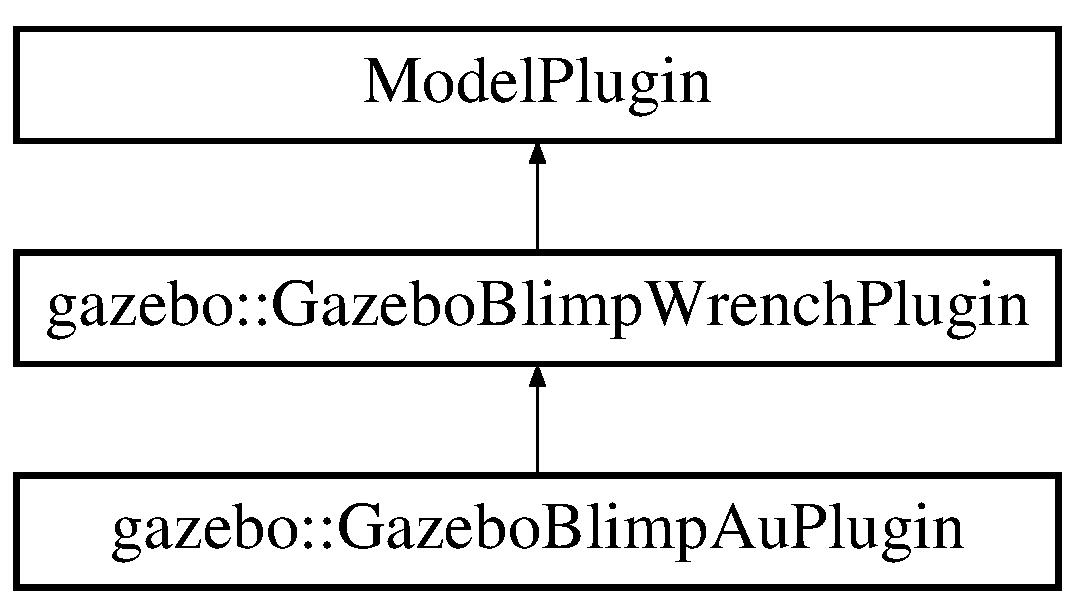
\includegraphics[height=3.000000cm]{classgazebo_1_1_gazebo_blimp_au_plugin}
\end{center}
\end{figure}
\subsection*{Protected Member Functions}
\begin{DoxyCompactItemize}
\item 
\hypertarget{classgazebo_1_1_gazebo_blimp_au_plugin_a55034cd0a7ef1e63f5fceea49ee96a9a}{void {\bfseries Load} (physics\-::\-Model\-Ptr \-\_\-model, sdf\-::\-Element\-Ptr \-\_\-sdf)}\label{classgazebo_1_1_gazebo_blimp_au_plugin_a55034cd0a7ef1e63f5fceea49ee96a9a}

\item 
\hypertarget{classgazebo_1_1_gazebo_blimp_au_plugin_a88959dd91977636408c6b48cc2eb9c21}{void {\bfseries Load\-Derived\-Class\-Params} (physics\-::\-Model\-Ptr \-\_\-model, sdf\-::\-Element\-Ptr \-\_\-sdf)}\label{classgazebo_1_1_gazebo_blimp_au_plugin_a88959dd91977636408c6b48cc2eb9c21}

\item 
\hypertarget{classgazebo_1_1_gazebo_blimp_au_plugin_ac04862eedaaf50d86b491c9b003c54c6}{void {\bfseries On\-Update} (const common\-::\-Update\-Info \&\-\_\-info)}\label{classgazebo_1_1_gazebo_blimp_au_plugin_ac04862eedaaf50d86b491c9b003c54c6}

\item 
\hypertarget{classgazebo_1_1_gazebo_blimp_au_plugin_a52c61d5436940937d8763f78c217bef3}{bool {\bfseries Set\-Force2\-D} (skye\-\_\-ros\-::\-Apply\-Force2\-D\-Cog\-Bf\-::\-Request \&req, skye\-\_\-ros\-::\-Apply\-Force2\-D\-Cog\-Bf\-::\-Response \&rep)}\label{classgazebo_1_1_gazebo_blimp_au_plugin_a52c61d5436940937d8763f78c217bef3}

\end{DoxyCompactItemize}
\subsection*{Protected Attributes}
\begin{DoxyCompactItemize}
\item 
\hypertarget{classgazebo_1_1_gazebo_blimp_au_plugin_a30314d64ec2363f60e074eb2cf1a3a35}{ros\-::\-Service\-Server {\bfseries server\-\_\-apply\-\_\-force\-\_\-2\-D\-\_\-bf\-\_\-}}\label{classgazebo_1_1_gazebo_blimp_au_plugin_a30314d64ec2363f60e074eb2cf1a3a35}

\item 
\hypertarget{classgazebo_1_1_gazebo_blimp_au_plugin_ac06fcb574c0541f9e1a88f38d6504315}{double {\bfseries prev\-\_\-sim\-\_\-time\-\_\-}}\label{classgazebo_1_1_gazebo_blimp_au_plugin_ac06fcb574c0541f9e1a88f38d6504315}

\item 
\hypertarget{classgazebo_1_1_gazebo_blimp_au_plugin_a296655d6cc4027e3919e1ada616c9f54}{double {\bfseries sampling\-\_\-time\-\_\-}}\label{classgazebo_1_1_gazebo_blimp_au_plugin_a296655d6cc4027e3919e1ada616c9f54}

\end{DoxyCompactItemize}


The documentation for this class was generated from the following files\-:\begin{DoxyCompactItemize}
\item 
skye\-\_\-ros/include/skye\-\_\-ros/gazebo\-\_\-blimp\-\_\-au\-\_\-plugin.\-h\item 
skye\-\_\-ros/src/gazebo\-\_\-blimp\-\_\-au\-\_\-plugin.\-cpp\end{DoxyCompactItemize}

\hypertarget{classgazebo_1_1_gazebo_blimp_dynamics_plugin}{\section{gazebo\-:\-:Gazebo\-Blimp\-Dynamics\-Plugin Class Reference}
\label{classgazebo_1_1_gazebo_blimp_dynamics_plugin}\index{gazebo\-::\-Gazebo\-Blimp\-Dynamics\-Plugin@{gazebo\-::\-Gazebo\-Blimp\-Dynamics\-Plugin}}
}
Inheritance diagram for gazebo\-:\-:Gazebo\-Blimp\-Dynamics\-Plugin\-:\begin{figure}[H]
\begin{center}
\leavevmode
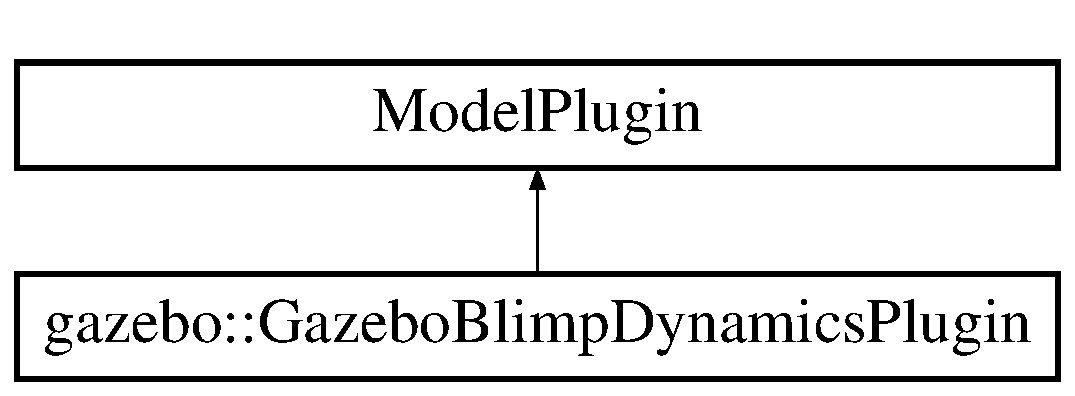
\includegraphics[height=2.000000cm]{classgazebo_1_1_gazebo_blimp_dynamics_plugin}
\end{center}
\end{figure}
\subsection*{Protected Member Functions}
\begin{DoxyCompactItemize}
\item 
\hypertarget{classgazebo_1_1_gazebo_blimp_dynamics_plugin_a3d0cbd15fdee85e1b1d2a5ee0962bc6b}{void {\bfseries Load} (physics\-::\-Model\-Ptr \-\_\-model, sdf\-::\-Element\-Ptr \-\_\-sdf)}\label{classgazebo_1_1_gazebo_blimp_dynamics_plugin_a3d0cbd15fdee85e1b1d2a5ee0962bc6b}

\item 
\hypertarget{classgazebo_1_1_gazebo_blimp_dynamics_plugin_aaa96cafa6a1d76eefd9f419806fadb24}{void {\bfseries Update\-Aerodynamic\-Forces} (const common\-::\-Update\-Info \&)}\label{classgazebo_1_1_gazebo_blimp_dynamics_plugin_aaa96cafa6a1d76eefd9f419806fadb24}

\end{DoxyCompactItemize}


The documentation for this class was generated from the following files\-:\begin{DoxyCompactItemize}
\item 
skye\-\_\-ros/include/skye\-\_\-ros/gazebo\-\_\-blimp\-\_\-dynamics\-\_\-plugin.\-h\item 
skye\-\_\-ros/src/gazebo\-\_\-blimp\-\_\-dynamics\-\_\-plugin.\-cpp\end{DoxyCompactItemize}

\hypertarget{classgazebo_1_1_gazebo_blimp_wrench_plugin}{\section{gazebo\-:\-:Gazebo\-Blimp\-Wrench\-Plugin Class Reference}
\label{classgazebo_1_1_gazebo_blimp_wrench_plugin}\index{gazebo\-::\-Gazebo\-Blimp\-Wrench\-Plugin@{gazebo\-::\-Gazebo\-Blimp\-Wrench\-Plugin}}
}
Inheritance diagram for gazebo\-:\-:Gazebo\-Blimp\-Wrench\-Plugin\-:\begin{figure}[H]
\begin{center}
\leavevmode
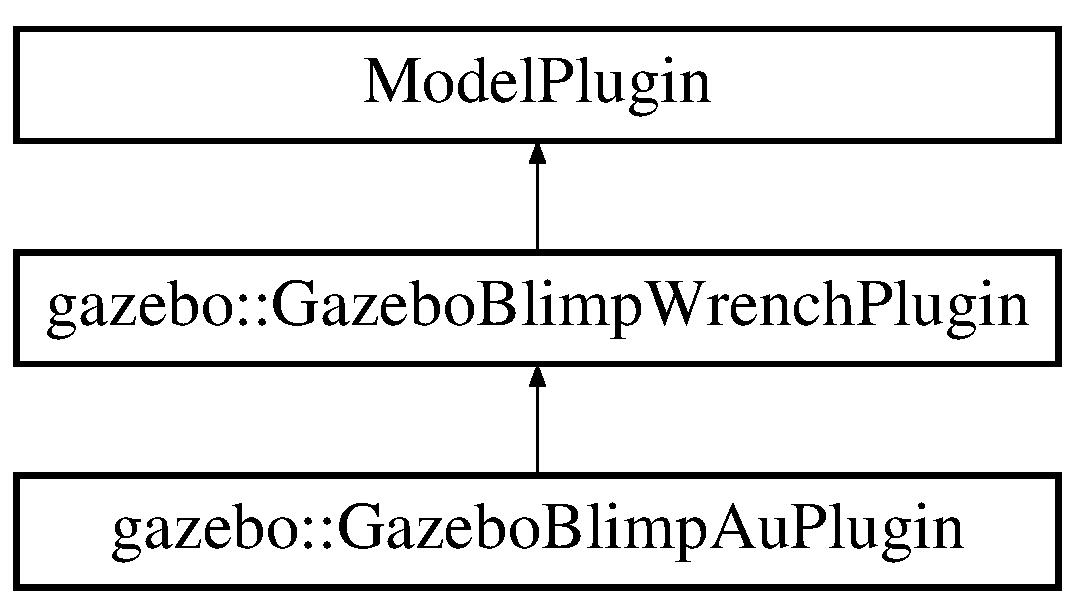
\includegraphics[height=3.000000cm]{classgazebo_1_1_gazebo_blimp_wrench_plugin}
\end{center}
\end{figure}
\subsection*{Protected Member Functions}
\begin{DoxyCompactItemize}
\item 
\hypertarget{classgazebo_1_1_gazebo_blimp_wrench_plugin_a4636030577d7e57f36ac6e02b7bcad98}{void {\bfseries Load} (physics\-::\-Model\-Ptr \-\_\-model, sdf\-::\-Element\-Ptr \-\_\-sdf)}\label{classgazebo_1_1_gazebo_blimp_wrench_plugin_a4636030577d7e57f36ac6e02b7bcad98}

\item 
\hypertarget{classgazebo_1_1_gazebo_blimp_wrench_plugin_a6b157a3315f7d10e0f07894f05edce90}{void {\bfseries Load\-Base\-Class\-Params} (physics\-::\-Model\-Ptr \-\_\-model, sdf\-::\-Element\-Ptr \-\_\-sdf)}\label{classgazebo_1_1_gazebo_blimp_wrench_plugin_a6b157a3315f7d10e0f07894f05edce90}

\item 
\hypertarget{classgazebo_1_1_gazebo_blimp_wrench_plugin_a1d9a1b19accceeb7c6eb7256b4d9070f}{bool {\bfseries Set\-Wrench} (skye\-\_\-ros\-::\-Apply\-Wrench\-Cog\-Bf\-::\-Request \&req, skye\-\_\-ros\-::\-Apply\-Wrench\-Cog\-Bf\-::\-Response \&rep)}\label{classgazebo_1_1_gazebo_blimp_wrench_plugin_a1d9a1b19accceeb7c6eb7256b4d9070f}

\item 
\hypertarget{classgazebo_1_1_gazebo_blimp_wrench_plugin_a290e3c882facc530446084c3a810c6c2}{bool {\bfseries Set\-Force} (skye\-\_\-ros\-::\-Apply\-Force\-Bf\-::\-Request \&req, skye\-\_\-ros\-::\-Apply\-Force\-Bf\-::\-Response \&rep)}\label{classgazebo_1_1_gazebo_blimp_wrench_plugin_a290e3c882facc530446084c3a810c6c2}

\item 
\hypertarget{classgazebo_1_1_gazebo_blimp_wrench_plugin_af4e6c14a01e2c9365aa508d7823c67b5}{bool {\bfseries Set\-Torque} (skye\-\_\-ros\-::\-Apply\-Torque\-Bf\-::\-Request \&req, skye\-\_\-ros\-::\-Apply\-Torque\-Bf\-::\-Response \&rep)}\label{classgazebo_1_1_gazebo_blimp_wrench_plugin_af4e6c14a01e2c9365aa508d7823c67b5}

\item 
\hypertarget{classgazebo_1_1_gazebo_blimp_wrench_plugin_ab7679050ec2c1f4f7b75b3889cdec6c8}{void {\bfseries On\-Update} (const common\-::\-Update\-Info \&)}\label{classgazebo_1_1_gazebo_blimp_wrench_plugin_ab7679050ec2c1f4f7b75b3889cdec6c8}

\item 
\hypertarget{classgazebo_1_1_gazebo_blimp_wrench_plugin_aab9fb73bade52597f7070bb8faef7378}{{\footnotesize template$<$class T $>$ }\\bool {\bfseries Check\-Vector3} (const T \&v)}\label{classgazebo_1_1_gazebo_blimp_wrench_plugin_aab9fb73bade52597f7070bb8faef7378}

\item 
\hypertarget{classgazebo_1_1_gazebo_blimp_wrench_plugin_a18dca12127345776b9e966f18c72b4a7}{{\footnotesize template$<$class In , class Out $>$ }\\void {\bfseries Copy\-Vector3} (const In \&v, Out \&v\-\_\-out)}\label{classgazebo_1_1_gazebo_blimp_wrench_plugin_a18dca12127345776b9e966f18c72b4a7}

\end{DoxyCompactItemize}
\subsection*{Protected Attributes}
\begin{DoxyCompactItemize}
\item 
\hypertarget{classgazebo_1_1_gazebo_blimp_wrench_plugin_adf20fff77602405801e8e77ed9e71610}{std\-::string {\bfseries namespace\-\_\-}}\label{classgazebo_1_1_gazebo_blimp_wrench_plugin_adf20fff77602405801e8e77ed9e71610}

\item 
\hypertarget{classgazebo_1_1_gazebo_blimp_wrench_plugin_a8ed3db7f6b880c673c94836a233f6b69}{ros\-::\-Node\-Handle $\ast$ {\bfseries node\-\_\-handle\-\_\-}}\label{classgazebo_1_1_gazebo_blimp_wrench_plugin_a8ed3db7f6b880c673c94836a233f6b69}

\item 
\hypertarget{classgazebo_1_1_gazebo_blimp_wrench_plugin_a517958c3b6872922667d790230f8a3f8}{std\-::string {\bfseries frame\-\_\-id\-\_\-}}\label{classgazebo_1_1_gazebo_blimp_wrench_plugin_a517958c3b6872922667d790230f8a3f8}

\item 
\hypertarget{classgazebo_1_1_gazebo_blimp_wrench_plugin_ad7020cd6f546ff529e524c54dc0bb7f5}{std\-::string {\bfseries link\-\_\-name\-\_\-}}\label{classgazebo_1_1_gazebo_blimp_wrench_plugin_ad7020cd6f546ff529e524c54dc0bb7f5}

\item 
\hypertarget{classgazebo_1_1_gazebo_blimp_wrench_plugin_aecdbcdba82e2de9cc92ce80035e40dfc}{physics\-::\-World\-Ptr {\bfseries world\-\_\-}}\label{classgazebo_1_1_gazebo_blimp_wrench_plugin_aecdbcdba82e2de9cc92ce80035e40dfc}

\item 
\hypertarget{classgazebo_1_1_gazebo_blimp_wrench_plugin_afe1ee435ae12574f11b61620189f4937}{physics\-::\-Model\-Ptr {\bfseries model\-\_\-}}\label{classgazebo_1_1_gazebo_blimp_wrench_plugin_afe1ee435ae12574f11b61620189f4937}

\item 
\hypertarget{classgazebo_1_1_gazebo_blimp_wrench_plugin_a4fee8aac766ecbbf26c68776efd48bec}{physics\-::\-Link\-Ptr {\bfseries link\-\_\-}}\label{classgazebo_1_1_gazebo_blimp_wrench_plugin_a4fee8aac766ecbbf26c68776efd48bec}

\item 
\hypertarget{classgazebo_1_1_gazebo_blimp_wrench_plugin_afd2cca05fd37109c075987ab836fa16a}{event\-::\-Connection\-Ptr {\bfseries update\-Connection\-\_\-}}\label{classgazebo_1_1_gazebo_blimp_wrench_plugin_afd2cca05fd37109c075987ab836fa16a}

\item 
\hypertarget{classgazebo_1_1_gazebo_blimp_wrench_plugin_a96b17df9675778f1b88d521bd3c57285}{ros\-::\-Service\-Server {\bfseries server\-\_\-apply\-\_\-wrench\-\_\-bf\-\_\-}}\label{classgazebo_1_1_gazebo_blimp_wrench_plugin_a96b17df9675778f1b88d521bd3c57285}

\item 
\hypertarget{classgazebo_1_1_gazebo_blimp_wrench_plugin_a24abb65b507037e39496e0a547fff35e}{ros\-::\-Service\-Server {\bfseries server\-\_\-apply\-\_\-force\-\_\-bf\-\_\-}}\label{classgazebo_1_1_gazebo_blimp_wrench_plugin_a24abb65b507037e39496e0a547fff35e}

\item 
\hypertarget{classgazebo_1_1_gazebo_blimp_wrench_plugin_aba3ea147fbe414d75290965c091ed3da}{ros\-::\-Service\-Server {\bfseries server\-\_\-apply\-\_\-torque\-\_\-bf\-\_\-}}\label{classgazebo_1_1_gazebo_blimp_wrench_plugin_aba3ea147fbe414d75290965c091ed3da}

\item 
\hypertarget{classgazebo_1_1_gazebo_blimp_wrench_plugin_a68fe0801ac4b3f9ccdd3fa573bf2147e}{\hyperlink{classgazebo_1_1_gazebo_body_wrench}{Gazebo\-Body\-Wrench} $\ast$ {\bfseries body\-\_\-wrench\-\_\-}}\label{classgazebo_1_1_gazebo_blimp_wrench_plugin_a68fe0801ac4b3f9ccdd3fa573bf2147e}

\end{DoxyCompactItemize}


The documentation for this class was generated from the following files\-:\begin{DoxyCompactItemize}
\item 
skye\-\_\-ros/include/skye\-\_\-ros/gazebo\-\_\-blimp\-\_\-wrench\-\_\-plugin.\-h\item 
skye\-\_\-ros/src/gazebo\-\_\-blimp\-\_\-wrench\-\_\-plugin.\-cpp\end{DoxyCompactItemize}

\hypertarget{classgazebo_1_1_gazebo_body_wrench}{\section{gazebo\-:\-:Gazebo\-Body\-Wrench Class Reference}
\label{classgazebo_1_1_gazebo_body_wrench}\index{gazebo\-::\-Gazebo\-Body\-Wrench@{gazebo\-::\-Gazebo\-Body\-Wrench}}
}
\subsection*{Public Member Functions}
\begin{DoxyCompactItemize}
\item 
\hypertarget{classgazebo_1_1_gazebo_body_wrench_a984289511dfcf80edc860b523a809953}{{\bfseries Gazebo\-Body\-Wrench} (const physics\-::\-World\-Ptr \&world, const gazebo\-::physics\-::\-Link\-Ptr \&body, const gazebo\-::math\-::\-Vector3 \&force\-\_\-application\-\_\-point)}\label{classgazebo_1_1_gazebo_body_wrench_a984289511dfcf80edc860b523a809953}

\item 
\hypertarget{classgazebo_1_1_gazebo_body_wrench_af17d57ca04935917517831f3f502997a}{{\bfseries Gazebo\-Body\-Wrench} (const physics\-::\-World\-Ptr \&world, const gazebo\-::physics\-::\-Link\-Ptr \&body)}\label{classgazebo_1_1_gazebo_body_wrench_af17d57ca04935917517831f3f502997a}

\item 
\hypertarget{classgazebo_1_1_gazebo_body_wrench_a266741da47bedeedb15b7bc43ef53188}{void {\bfseries Apply\-Wrench} ()}\label{classgazebo_1_1_gazebo_body_wrench_a266741da47bedeedb15b7bc43ef53188}

\item 
\hypertarget{classgazebo_1_1_gazebo_body_wrench_aa25dd4548ae87b8b3d23ea922d8a0f9e}{void {\bfseries Update\-No\-Filter} ()}\label{classgazebo_1_1_gazebo_body_wrench_aa25dd4548ae87b8b3d23ea922d8a0f9e}

\item 
\hypertarget{classgazebo_1_1_gazebo_body_wrench_a9c35669b56e1d9640cddc1fccf93bd7f}{void {\bfseries Update\-Filter} (const double \&sampling\-\_\-time)}\label{classgazebo_1_1_gazebo_body_wrench_a9c35669b56e1d9640cddc1fccf93bd7f}

\item 
\hypertarget{classgazebo_1_1_gazebo_body_wrench_a8ba355bad85027cd7cc1c15131d8e792}{void {\bfseries Set\-Body\-Wrench} (const gazebo\-::math\-::\-Vector3 \&force, const gazebo\-::math\-::\-Vector3 \&torque, const ros\-::\-Time \&start\-\_\-time, const ros\-::\-Duration \&duration)}\label{classgazebo_1_1_gazebo_body_wrench_a8ba355bad85027cd7cc1c15131d8e792}

\item 
\hypertarget{classgazebo_1_1_gazebo_body_wrench_a22da3c17fbf8cf202bcb62a77c3707d6}{void {\bfseries Set\-Body\-Force} (const gazebo\-::math\-::\-Vector3 \&force, const ros\-::\-Time \&start\-\_\-time, const ros\-::\-Duration \&duration)}\label{classgazebo_1_1_gazebo_body_wrench_a22da3c17fbf8cf202bcb62a77c3707d6}

\item 
\hypertarget{classgazebo_1_1_gazebo_body_wrench_ab672b6b39276477b3bb61586cfa321dd}{void {\bfseries Set\-Body\-Torque} (const gazebo\-::math\-::\-Vector3 \&torque, const ros\-::\-Time \&start\-\_\-time, const ros\-::\-Duration \&duration)}\label{classgazebo_1_1_gazebo_body_wrench_ab672b6b39276477b3bb61586cfa321dd}

\item 
\hypertarget{classgazebo_1_1_gazebo_body_wrench_a51b0f72347b899b9c973abae1f6a4fc1}{void {\bfseries Set\-Start\-Time} (const ros\-::\-Time \&t\-\_\-user, ros\-::\-Time \&t\-\_\-out)}\label{classgazebo_1_1_gazebo_body_wrench_a51b0f72347b899b9c973abae1f6a4fc1}

\item 
\hypertarget{classgazebo_1_1_gazebo_body_wrench_a7b81e76da9e7d3f5653f3c0b21504424}{void {\bfseries Set\-Filters\-Matrices} (const Eigen\-::\-Ref$<$ const Eigen\-::\-Matrix$<$ double, 1, 1 $>$ $>$ \&A\-\_\-orientation, const Eigen\-::\-Ref$<$ const Eigen\-::\-Matrix$<$ double, 1, 1 $>$ $>$ \&B\-\_\-orientation, const Eigen\-::\-Ref$<$ const Eigen\-::\-Matrix$<$ double, 2, 2 $>$ $>$ \&A\-\_\-thrust, const Eigen\-::\-Ref$<$ const Eigen\-::\-Matrix$<$ double, 2, 1 $>$ $>$ \&B\-\_\-thrust)}\label{classgazebo_1_1_gazebo_body_wrench_a7b81e76da9e7d3f5653f3c0b21504424}

\item 
\hypertarget{classgazebo_1_1_gazebo_body_wrench_af08623ecc1f490f71b46ce508b4f0808}{bool {\bfseries Apply\-Vector} (const ros\-::\-Time \&start\-\_\-time, const ros\-::\-Duration \&duration)}\label{classgazebo_1_1_gazebo_body_wrench_af08623ecc1f490f71b46ce508b4f0808}

\end{DoxyCompactItemize}


The documentation for this class was generated from the following files\-:\begin{DoxyCompactItemize}
\item 
skye\-\_\-ros/include/skye\-\_\-ros/gazebo\-\_\-body\-\_\-wrench.\-h\item 
skye\-\_\-ros/src/gazebo\-\_\-body\-\_\-wrench.\-cpp\end{DoxyCompactItemize}

\hypertarget{class_pose_controller_node}{\section{Pose\-Controller\-Node Class Reference}
\label{class_pose_controller_node}\index{Pose\-Controller\-Node@{Pose\-Controller\-Node}}
}
\subsection*{Public Member Functions}
\begin{DoxyCompactItemize}
\item 
\hyperlink{class_pose_controller_node_a17466a8314ad354402401ba27157594c}{Pose\-Controller\-Node} (ros\-::\-Node\-Handle nh)
\begin{DoxyCompactList}\small\item\em \hyperlink{class_pose_controller_node}{Pose\-Controller\-Node} \-: the constructor initializes the dynamic parameters, creates the desired controller sets up the service to control skye. \end{DoxyCompactList}\item 
void \hyperlink{class_pose_controller_node_aab9762d618a38b99cbfbcaecd2163606}{Config\-Callback} (const skye\-\_\-controls\-::skye\-\_\-params\-Config \&config, uint32\-\_\-t level)
\begin{DoxyCompactList}\small\item\em Config\-Callback \-: Callback for the dynamic configuration of the parameters. \end{DoxyCompactList}\item 
void \hyperlink{class_pose_controller_node_ac4582290cf6ff6b5cd9564fd386c3b39}{Position\-Callback} (const gazebo\-\_\-msgs\-::\-Link\-State\-::\-Const\-Ptr \&msg)
\begin{DoxyCompactList}\small\item\em Position\-Callback \-: this callback is called by the topic providing \hyperlink{class_skye}{Skye}'s ground truth. \end{DoxyCompactList}\item 
void \hyperlink{class_pose_controller_node_a1804624b5c2f57b08fcd1c50b8118cd7}{Angular\-Velocity\-Callback} (const sensor\-\_\-msgs\-::\-Imu\-::\-Const\-Ptr \&msg)
\begin{DoxyCompactList}\small\item\em Angular\-Velocity\-Callback \-: this callback receives the angular velocity from the I\-M\-U. \end{DoxyCompactList}\item 
bool \hyperlink{class_pose_controller_node_a0b12265a62dad33caa6063f5cb582c80}{Call\-Service} ()
\begin{DoxyCompactList}\small\item\em Call\-Service \-: utility wrapped function to call the service. \end{DoxyCompactList}\end{DoxyCompactItemize}


\subsection{Constructor \& Destructor Documentation}
\hypertarget{class_pose_controller_node_a17466a8314ad354402401ba27157594c}{\index{Pose\-Controller\-Node@{Pose\-Controller\-Node}!Pose\-Controller\-Node@{Pose\-Controller\-Node}}
\index{Pose\-Controller\-Node@{Pose\-Controller\-Node}!PoseControllerNode@{Pose\-Controller\-Node}}
\subsubsection[{Pose\-Controller\-Node}]{\setlength{\rightskip}{0pt plus 5cm}Pose\-Controller\-Node\-::\-Pose\-Controller\-Node (
\begin{DoxyParamCaption}
\item[{ros\-::\-Node\-Handle}]{nh}
\end{DoxyParamCaption}
)}}\label{class_pose_controller_node_a17466a8314ad354402401ba27157594c}


\hyperlink{class_pose_controller_node}{Pose\-Controller\-Node} \-: the constructor initializes the dynamic parameters, creates the desired controller sets up the service to control skye. 


\begin{DoxyParams}{Parameters}
{\em nh} & \-: Ros node handle to create the service\\
\hline
\end{DoxyParams}
The constructor has a fixed service name that is saved as a class member in the main function. The successful creation of this node is conditioned upon succesfully finding the service. In case the service is wrong or not published the node does not created. The dynamic parameters are used for dynamically configure control parameters 

\subsection{Member Function Documentation}
\hypertarget{class_pose_controller_node_a1804624b5c2f57b08fcd1c50b8118cd7}{\index{Pose\-Controller\-Node@{Pose\-Controller\-Node}!Angular\-Velocity\-Callback@{Angular\-Velocity\-Callback}}
\index{Angular\-Velocity\-Callback@{Angular\-Velocity\-Callback}!PoseControllerNode@{Pose\-Controller\-Node}}
\subsubsection[{Angular\-Velocity\-Callback}]{\setlength{\rightskip}{0pt plus 5cm}void Pose\-Controller\-Node\-::\-Angular\-Velocity\-Callback (
\begin{DoxyParamCaption}
\item[{const sensor\-\_\-msgs\-::\-Imu\-::\-Const\-Ptr \&}]{msg}
\end{DoxyParamCaption}
)}}\label{class_pose_controller_node_a1804624b5c2f57b08fcd1c50b8118cd7}


Angular\-Velocity\-Callback \-: this callback receives the angular velocity from the I\-M\-U. 


\begin{DoxyParams}{Parameters}
{\em msg} & \-: the imu message containing angular velocity \\
\hline
\end{DoxyParams}
\hypertarget{class_pose_controller_node_a0b12265a62dad33caa6063f5cb582c80}{\index{Pose\-Controller\-Node@{Pose\-Controller\-Node}!Call\-Service@{Call\-Service}}
\index{Call\-Service@{Call\-Service}!PoseControllerNode@{Pose\-Controller\-Node}}
\subsubsection[{Call\-Service}]{\setlength{\rightskip}{0pt plus 5cm}bool Pose\-Controller\-Node\-::\-Call\-Service (
\begin{DoxyParamCaption}
{}
\end{DoxyParamCaption}
)}}\label{class_pose_controller_node_a0b12265a62dad33caa6063f5cb582c80}


Call\-Service \-: utility wrapped function to call the service. 

\begin{DoxyReturn}{Returns}
\-: true if the service was called correctly 
\end{DoxyReturn}
\hypertarget{class_pose_controller_node_aab9762d618a38b99cbfbcaecd2163606}{\index{Pose\-Controller\-Node@{Pose\-Controller\-Node}!Config\-Callback@{Config\-Callback}}
\index{Config\-Callback@{Config\-Callback}!PoseControllerNode@{Pose\-Controller\-Node}}
\subsubsection[{Config\-Callback}]{\setlength{\rightskip}{0pt plus 5cm}void Pose\-Controller\-Node\-::\-Config\-Callback (
\begin{DoxyParamCaption}
\item[{const skye\-\_\-controls\-::skye\-\_\-params\-Config \&}]{config, }
\item[{uint32\-\_\-t}]{level}
\end{DoxyParamCaption}
)}}\label{class_pose_controller_node_aab9762d618a38b99cbfbcaecd2163606}


Config\-Callback \-: Callback for the dynamic configuration of the parameters. 


\begin{DoxyParams}{Parameters}
{\em config} & \-: the skye\-\_\-params congifuration file \\
\hline
{\em level} & \-: not used \\
\hline
\end{DoxyParams}
\hypertarget{class_pose_controller_node_ac4582290cf6ff6b5cd9564fd386c3b39}{\index{Pose\-Controller\-Node@{Pose\-Controller\-Node}!Position\-Callback@{Position\-Callback}}
\index{Position\-Callback@{Position\-Callback}!PoseControllerNode@{Pose\-Controller\-Node}}
\subsubsection[{Position\-Callback}]{\setlength{\rightskip}{0pt plus 5cm}void Pose\-Controller\-Node\-::\-Position\-Callback (
\begin{DoxyParamCaption}
\item[{const gazebo\-\_\-msgs\-::\-Link\-State\-::\-Const\-Ptr \&}]{msg}
\end{DoxyParamCaption}
)}}\label{class_pose_controller_node_ac4582290cf6ff6b5cd9564fd386c3b39}


Position\-Callback \-: this callback is called by the topic providing \hyperlink{class_skye}{Skye}'s ground truth. 


\begin{DoxyParams}{Parameters}
{\em msg} & \-: the message containing the lik state This is used as callback to perform the control loop, which means that control inputs are applied every time a new linkstate is received. \\
\hline
\end{DoxyParams}


The documentation for this class was generated from the following files\-:\begin{DoxyCompactItemize}
\item 
skye\-\_\-controls/src/node/pose\-\_\-control\-\_\-node.\-h\item 
skye\-\_\-controls/src/node/pose\-\_\-control\-\_\-node.\-cpp\end{DoxyCompactItemize}

\hypertarget{structskye__ros_1_1skye__ros__parameters}{\section{skye\-\_\-ros\-:\-:skye\-\_\-ros\-\_\-parameters Struct Reference}
\label{structskye__ros_1_1skye__ros__parameters}\index{skye\-\_\-ros\-::skye\-\_\-ros\-\_\-parameters@{skye\-\_\-ros\-::skye\-\_\-ros\-\_\-parameters}}
}
\subsection*{Public Attributes}
\begin{DoxyCompactItemize}
\item 
\hypertarget{structskye__ros_1_1skye__ros__parameters_abc91bf8157ed23bf70513961c8f21ef8}{std\-::string {\bfseries topic\-\_\-imu\-\_\-gazebo}}\label{structskye__ros_1_1skye__ros__parameters_abc91bf8157ed23bf70513961c8f21ef8}

\item 
\hypertarget{structskye__ros_1_1skye__ros__parameters_ad9a6f627926b8ba9c8895b5f9857cce9}{std\-::string {\bfseries topic\-\_\-imu\-\_\-skye}}\label{structskye__ros_1_1skye__ros__parameters_ad9a6f627926b8ba9c8895b5f9857cce9}

\item 
\hypertarget{structskye__ros_1_1skye__ros__parameters_aa867963d220c8d3bdce8871487d20ffb}{std\-::string {\bfseries topic\-\_\-ground\-\_\-truth\-\_\-hull}}\label{structskye__ros_1_1skye__ros__parameters_aa867963d220c8d3bdce8871487d20ffb}

\item 
\hypertarget{structskye__ros_1_1skye__ros__parameters_a0512980e99daf77a15c9fb62744cb819}{std\-::string {\bfseries service\-\_\-get\-\_\-link\-\_\-state}}\label{structskye__ros_1_1skye__ros__parameters_a0512980e99daf77a15c9fb62744cb819}

\item 
\hypertarget{structskye__ros_1_1skye__ros__parameters_a9474c6e4c132b4a9f3c0287ccb8df1d0}{double {\bfseries hull\-\_\-ground\-\_\-truth\-\_\-update\-\_\-frequency}}\label{structskye__ros_1_1skye__ros__parameters_a9474c6e4c132b4a9f3c0287ccb8df1d0}

\item 
\hypertarget{structskye__ros_1_1skye__ros__parameters_adfece757e4b6692b2622be816c5e2450}{std\-::string {\bfseries blimp\-\_\-name}}\label{structskye__ros_1_1skye__ros__parameters_adfece757e4b6692b2622be816c5e2450}

\item 
\hypertarget{structskye__ros_1_1skye__ros__parameters_aa13dc5a1696b1ca9f5b14437a6282f1a}{std\-::string {\bfseries hull\-\_\-name}}\label{structskye__ros_1_1skye__ros__parameters_aa13dc5a1696b1ca9f5b14437a6282f1a}

\end{DoxyCompactItemize}


The documentation for this struct was generated from the following file\-:\begin{DoxyCompactItemize}
\item 
skye\-\_\-ros/include/skye\-\_\-ros/skye\-\_\-ros.\-h\end{DoxyCompactItemize}

\hypertarget{class_skye_geometric_controller}{\section{Skye\-Geometric\-Controller Class Reference}
\label{class_skye_geometric_controller}\index{Skye\-Geometric\-Controller@{Skye\-Geometric\-Controller}}
}
\subsection*{Public Member Functions}
\begin{DoxyCompactItemize}
\item 
\hypertarget{class_skye_geometric_controller_a40739735f7c55b861647ecad873080ac}{\hyperlink{class_skye_geometric_controller_a40739735f7c55b861647ecad873080ac}{Skye\-Geometric\-Controller} ()}\label{class_skye_geometric_controller_a40739735f7c55b861647ecad873080ac}

\begin{DoxyCompactList}\small\item\em \hyperlink{class_skye_geometric_controller_a40739735f7c55b861647ecad873080ac}{Skye\-Geometric\-Controller\-::\-Skye\-Geometric\-Controller} Just creates the object. \end{DoxyCompactList}\item 
void \hyperlink{class_skye_geometric_controller_a78773edf4b0a80b1e26daec62b17a42a}{Initialize\-Params} (const \hyperlink{struct_skye_parameters}{Skye\-Parameters} param)
\begin{DoxyCompactList}\small\item\em Initialize\-Params \-: function that initializes all the parameters needed by the controller. \end{DoxyCompactList}\item 
void \hyperlink{class_skye_geometric_controller_a59e2b48fa22a5910cf932cd8217ae062}{Update\-Parameters} (const Eigen\-::\-Vector3d \&poisiton\-\_\-if, const Eigen\-::\-Vector3d \&velocity\-\_\-if, const Eigen\-::\-Quaterniond \&orientation\-\_\-bf, const Eigen\-::\-Vector3d \&a\-\_\-angular\-\_\-velocity\-\_\-bf)
\begin{DoxyCompactList}\small\item\em Update\-Parameters \-: updates the parameters for control errors. \end{DoxyCompactList}\item 
void \hyperlink{class_skye_geometric_controller_a86e1970fa9f94b0a1d09b7368ee19bf8}{Update\-Gains} (double k\-\_\-x, double k\-\_\-v, double k\-\_\-if, double k\-\_\-im, double k\-\_\-\-R, double k\-\_\-omega)
\begin{DoxyCompactList}\small\item\em Update\-Gains \-: Provides an interface to dynamically change control parameters. \end{DoxyCompactList}\item 
void \hyperlink{class_skye_geometric_controller_afe9b74936a7118f7185113db56954f73}{Compute\-Force} (Eigen\-::\-Vector3d $\ast$output\-\_\-force\-\_\-bf)
\begin{DoxyCompactList}\small\item\em Compute\-Force \-: computes the force to control the position of Skye. \end{DoxyCompactList}\item 
void \hyperlink{class_skye_geometric_controller_ab2676ca5ec54b90946bd2707abc39872}{Compute\-Acceleration} (Eigen\-::\-Vector3d $\ast$output\-\_\-acceleration\-\_\-bf)
\begin{DoxyCompactList}\small\item\em Compute\-Acceleration \-: computes the momentum to control the orientation of Skye. \end{DoxyCompactList}\item 
void \hyperlink{class_skye_geometric_controller_a47c430b43ad57b8c9ade33d36b2f7ffe}{Update\-Desired\-Pose} (const Eigen\-::\-Vector3d \&desired\-\_\-position\-\_\-if, const Eigen\-::\-Vector3d \&desired\-\_\-velocity\-\_\-if, const Eigen\-::\-Vector3d \&desired\-\_\-angular\-\_\-velocity\-\_\-bf, const Eigen\-::\-Vector3d \&desired\-\_\-acceleration\-\_\-if, const Eigen\-::\-Quaterniond \&desired\-\_\-orientation\-\_\-bf)
\begin{DoxyCompactList}\small\item\em Update\-Desired\-Pose \-: updates the desired pose of Skye for new control iteration. \end{DoxyCompactList}\end{DoxyCompactItemize}
\subsection*{Private Member Functions}
\begin{DoxyCompactItemize}
\item 
void \hyperlink{class_skye_geometric_controller_a7b662c7331963aedd0d978ee13ce222e}{Vector\-From\-Skew\-Matrix} (Eigen\-::\-Matrix3d \&skew\-\_\-matrix, Eigen\-::\-Vector3d $\ast$vector)
\begin{DoxyCompactList}\small\item\em Vector\-From\-Skew\-Matrix \-: returns a vector from a skew matrix. \end{DoxyCompactList}\item 
\hypertarget{class_skye_geometric_controller_a360748121b002192b1019a7fd325dfd5}{void \hyperlink{class_skye_geometric_controller_a360748121b002192b1019a7fd325dfd5}{Compute\-Normalized\-Gains} ()}\label{class_skye_geometric_controller_a360748121b002192b1019a7fd325dfd5}

\begin{DoxyCompactList}\small\item\em \hyperlink{class_skye_geometric_controller_a360748121b002192b1019a7fd325dfd5}{Skye\-Geometric\-Controller\-::\-Compute\-Normalized\-Gains} \-: normalizes the gains with the inertia of Skye in order to have inertia-\/independent calculations. \end{DoxyCompactList}\item 
void \hyperlink{class_skye_geometric_controller_a75b38d5fe2687493eb6c0e917fc0fa1a}{Saturate\-Vector} (double a\-\_\-threshold, Eigen\-::\-Vector3d $\ast$a\-\_\-vector)
\begin{DoxyCompactList}\small\item\em Saturate\-Vector \-: small utility that saturates a vector component-\/wise given a threshold. \end{DoxyCompactList}\end{DoxyCompactItemize}
\subsection*{Private Attributes}
\begin{DoxyCompactItemize}
\item 
\hypertarget{class_skye_geometric_controller_ab5e7e12358398de48747ffec05b779a4}{bool \hyperlink{class_skye_geometric_controller_ab5e7e12358398de48747ffec05b779a4}{singularity\-\_\-detected\-\_\-}}\label{class_skye_geometric_controller_ab5e7e12358398de48747ffec05b779a4}

\begin{DoxyCompactList}\small\item\em singularity\-\_\-detected\-\_\- \-: boolean that shows wether there's been critical point \end{DoxyCompactList}\item 
\hypertarget{class_skye_geometric_controller_ac5b6e324aca728265c20590eae7492ad}{double \hyperlink{class_skye_geometric_controller_ac5b6e324aca728265c20590eae7492ad}{k\-\_\-x\-\_\-}}\label{class_skye_geometric_controller_ac5b6e324aca728265c20590eae7492ad}

\begin{DoxyCompactList}\small\item\em k\-\_\-x\-\_\- \-: the position control gain \end{DoxyCompactList}\item 
\hypertarget{class_skye_geometric_controller_a904f70d115099a3ab0bc7b1bb6e2d7c5}{double \hyperlink{class_skye_geometric_controller_a904f70d115099a3ab0bc7b1bb6e2d7c5}{k\-\_\-v\-\_\-}}\label{class_skye_geometric_controller_a904f70d115099a3ab0bc7b1bb6e2d7c5}

\begin{DoxyCompactList}\small\item\em k\-\_\-v\-\_\- \-: the linear velocity control gain \end{DoxyCompactList}\item 
\hypertarget{class_skye_geometric_controller_ad5bcb155689c05545076c0143a41b134}{double \hyperlink{class_skye_geometric_controller_ad5bcb155689c05545076c0143a41b134}{k\-\_\-if\-\_\-}}\label{class_skye_geometric_controller_ad5bcb155689c05545076c0143a41b134}

\begin{DoxyCompactList}\small\item\em k\-\_\-if\-\_\- \-: the force integrator control gain \end{DoxyCompactList}\item 
\hypertarget{class_skye_geometric_controller_a238e9820bbeab93244b9dc6c804c6529}{double \hyperlink{class_skye_geometric_controller_a238e9820bbeab93244b9dc6c804c6529}{k\-\_\-im\-\_\-}}\label{class_skye_geometric_controller_a238e9820bbeab93244b9dc6c804c6529}

\begin{DoxyCompactList}\small\item\em k\-\_\-im\-\_\- \-: the momentum integrator control gain \end{DoxyCompactList}\item 
\hypertarget{class_skye_geometric_controller_a86653a2b4757f45cd62862f167188e58}{double \hyperlink{class_skye_geometric_controller_a86653a2b4757f45cd62862f167188e58}{k\-\_\-omega\-\_\-}}\label{class_skye_geometric_controller_a86653a2b4757f45cd62862f167188e58}

\begin{DoxyCompactList}\small\item\em k\-\_\-omega\-\_\- \-: the angular velocity control gain \end{DoxyCompactList}\item 
\hypertarget{class_skye_geometric_controller_a9b851fbcdc2f38c99d95011902024100}{double \hyperlink{class_skye_geometric_controller_a9b851fbcdc2f38c99d95011902024100}{k\-\_\-\-R\-\_\-}}\label{class_skye_geometric_controller_a9b851fbcdc2f38c99d95011902024100}

\begin{DoxyCompactList}\small\item\em k\-\_\-\-R\-\_\- \-: the attitude control gain \end{DoxyCompactList}\item 
\hypertarget{class_skye_geometric_controller_af9681a8efa6c5ebfae8394539e6cdf01}{Eigen\-::\-Vector3d \hyperlink{class_skye_geometric_controller_af9681a8efa6c5ebfae8394539e6cdf01}{normalized\-\_\-k\-\_\-\-R\-\_\-}}\label{class_skye_geometric_controller_af9681a8efa6c5ebfae8394539e6cdf01}

\begin{DoxyCompactList}\small\item\em normalized\-\_\-k\-\_\-\-R\-\_\- \-: attitude control coefficients normalized with the inertia \end{DoxyCompactList}\item 
\hypertarget{class_skye_geometric_controller_a4346afc258d59ee51ec4726bc8f971fe}{Eigen\-::\-Vector3d \hyperlink{class_skye_geometric_controller_a4346afc258d59ee51ec4726bc8f971fe}{normalized\-\_\-k\-\_\-omega\-\_\-}}\label{class_skye_geometric_controller_a4346afc258d59ee51ec4726bc8f971fe}

\begin{DoxyCompactList}\small\item\em normalized\-\_\-k\-\_\-omega\-\_\- \-: angular velocity control coefficients normalized with the inertia \end{DoxyCompactList}\item 
\hypertarget{class_skye_geometric_controller_acd5d07ef7dcabd011a285a09d10d2bc9}{double \hyperlink{class_skye_geometric_controller_acd5d07ef7dcabd011a285a09d10d2bc9}{mass\-\_\-}}\label{class_skye_geometric_controller_acd5d07ef7dcabd011a285a09d10d2bc9}

\begin{DoxyCompactList}\small\item\em mass\-\_\- \-: Skye's Mass \end{DoxyCompactList}\item 
\hypertarget{class_skye_geometric_controller_a4e005727f2603f4dc2ff5c8dcdd3d22b}{double \hyperlink{class_skye_geometric_controller_a4e005727f2603f4dc2ff5c8dcdd3d22b}{radius\-\_\-}}\label{class_skye_geometric_controller_a4e005727f2603f4dc2ff5c8dcdd3d22b}

\begin{DoxyCompactList}\small\item\em radius\-\_\- \-: Skye's radius \end{DoxyCompactList}\item 
\hypertarget{class_skye_geometric_controller_aef174ecff7363b397b961b2663efe4b6}{int \hyperlink{class_skye_geometric_controller_aef174ecff7363b397b961b2663efe4b6}{number\-\_\-of\-\_\-actuators\-\_\-}}\label{class_skye_geometric_controller_aef174ecff7363b397b961b2663efe4b6}

\begin{DoxyCompactList}\small\item\em number\-\_\-of\-\_\-actuators\-\_\- \-: the number of actuators skye has. It is used to compute the momentum saturation \end{DoxyCompactList}\item 
\hypertarget{class_skye_geometric_controller_a20b4551b3e19acd625f490602afc0e28}{double \hyperlink{class_skye_geometric_controller_a20b4551b3e19acd625f490602afc0e28}{maximum\-\_\-force\-\_\-cog\-\_\-bf\-\_\-}}\label{class_skye_geometric_controller_a20b4551b3e19acd625f490602afc0e28}

\begin{DoxyCompactList}\small\item\em maximum\-\_\-force\-\_\-cog\-\_\-bf\-\_\- \-: unidirectional saturation value for the force \end{DoxyCompactList}\item 
\hypertarget{class_skye_geometric_controller_a39fcc2bc245a64623e72314b61fcae96}{double \hyperlink{class_skye_geometric_controller_a39fcc2bc245a64623e72314b61fcae96}{maximum\-\_\-acceleration\-\_\-cog\-\_\-bf\-\_\-}}\label{class_skye_geometric_controller_a39fcc2bc245a64623e72314b61fcae96}

\begin{DoxyCompactList}\small\item\em maximum\-\_\-acceleration\-\_\-cog\-\_\-bf\-\_\- \-: threshold close to the setpoint when to perform the windup \end{DoxyCompactList}\item 
\hypertarget{class_skye_geometric_controller_a616c2c91d56897116b1b424df07b836b}{double \hyperlink{class_skye_geometric_controller_a616c2c91d56897116b1b424df07b836b}{distance\-\_\-integrator\-\_\-treshold\-\_\-}}\label{class_skye_geometric_controller_a616c2c91d56897116b1b424df07b836b}

\begin{DoxyCompactList}\small\item\em distance\-\_\-integrator\-\_\-treshold\-\_\- \-: threshold under which the position integrator is activated \end{DoxyCompactList}\item 
\hypertarget{class_skye_geometric_controller_a5f57a2407c42b2018af12fbb4cf34489}{double \hyperlink{class_skye_geometric_controller_a5f57a2407c42b2018af12fbb4cf34489}{attitude\-\_\-integrator\-\_\-treshold\-\_\-}}\label{class_skye_geometric_controller_a5f57a2407c42b2018af12fbb4cf34489}

\begin{DoxyCompactList}\small\item\em attitude\-\_\-integrator\-\_\-treshold\-\_\- \-: threshold under which the attitude integrator is activated \end{DoxyCompactList}\item 
\hypertarget{class_skye_geometric_controller_a086297b4c26d21f8cd6207650de04c8f}{double \hyperlink{class_skye_geometric_controller_a086297b4c26d21f8cd6207650de04c8f}{maximum\-\_\-force\-\_\-integrator\-\_\-}}\label{class_skye_geometric_controller_a086297b4c26d21f8cd6207650de04c8f}

\begin{DoxyCompactList}\small\item\em maximum\-\_\-force\-\_\-integrator\-\_\- \-: saturation value for the position control integrator \end{DoxyCompactList}\item 
\hypertarget{class_skye_geometric_controller_adc4fc8031b2928436d455f68ae4c66f2}{double \hyperlink{class_skye_geometric_controller_adc4fc8031b2928436d455f68ae4c66f2}{maximum\-\_\-acceleration\-\_\-integrator\-\_\-}}\label{class_skye_geometric_controller_adc4fc8031b2928436d455f68ae4c66f2}

\begin{DoxyCompactList}\small\item\em maximum\-\_\-momentum\-\_\-integrator\-\_\- \-: saturation value for the attitude control integrator \end{DoxyCompactList}\item 
\hypertarget{class_skye_geometric_controller_a3da2aa99720a266392a2e5910ce38fa0}{Eigen\-::\-Vector3d \hyperlink{class_skye_geometric_controller_a3da2aa99720a266392a2e5910ce38fa0}{desired\-\_\-position\-\_\-if\-\_\-}}\label{class_skye_geometric_controller_a3da2aa99720a266392a2e5910ce38fa0}

\begin{DoxyCompactList}\small\item\em desired\-\_\-position\-\_\-if\-\_\- \-: desired position expressed in the inertial frame \end{DoxyCompactList}\item 
\hypertarget{class_skye_geometric_controller_a7a3a687ba05d79fe99b1c9b355d2c99d}{Eigen\-::\-Vector3d \hyperlink{class_skye_geometric_controller_a7a3a687ba05d79fe99b1c9b355d2c99d}{desired\-\_\-velocity\-\_\-if\-\_\-}}\label{class_skye_geometric_controller_a7a3a687ba05d79fe99b1c9b355d2c99d}

\begin{DoxyCompactList}\small\item\em desired\-\_\-velocity\-\_\-if\-\_\- \-: desired linear velocity expressed in the inertial frame \end{DoxyCompactList}\item 
\hypertarget{class_skye_geometric_controller_abaa48abd74ebc19730c665e769c7fd26}{Eigen\-::\-Vector3d \hyperlink{class_skye_geometric_controller_abaa48abd74ebc19730c665e769c7fd26}{desired\-\_\-acceleration\-\_\-if\-\_\-}}\label{class_skye_geometric_controller_abaa48abd74ebc19730c665e769c7fd26}

\begin{DoxyCompactList}\small\item\em desired\-\_\-acceleration\-\_\-if\-\_\- \-: desired linear acceleration expressed in the inertial frame \end{DoxyCompactList}\item 
\hypertarget{class_skye_geometric_controller_a2bf72b9a46d793c849ee8c5569eb8fd2}{Eigen\-::\-Vector3d \hyperlink{class_skye_geometric_controller_a2bf72b9a46d793c849ee8c5569eb8fd2}{desired\-\_\-angular\-\_\-velocity\-\_\-bf\-\_\-}}\label{class_skye_geometric_controller_a2bf72b9a46d793c849ee8c5569eb8fd2}

\begin{DoxyCompactList}\small\item\em desired\-\_\-angular\-\_\-velocity\-\_\-bf\-\_\- \-: desired angular velocity expressed in the body frame \end{DoxyCompactList}\item 
\hypertarget{class_skye_geometric_controller_a0d3d2af49252e08535ff312ed0c9b5ad}{Eigen\-::\-Vector3d \hyperlink{class_skye_geometric_controller_a0d3d2af49252e08535ff312ed0c9b5ad}{desired\-\_\-angular\-\_\-acceleration\-\_\-bf\-\_\-}}\label{class_skye_geometric_controller_a0d3d2af49252e08535ff312ed0c9b5ad}

\begin{DoxyCompactList}\small\item\em desired\-\_\-angular\-\_\-acceleration\-\_\-bf\-\_\- \-: desired angular acceleration expressed in the body frame \end{DoxyCompactList}\item 
\hypertarget{class_skye_geometric_controller_a6fcf8fba87d817dc4a810f58181af3bd}{Eigen\-::\-Vector3d \hyperlink{class_skye_geometric_controller_a6fcf8fba87d817dc4a810f58181af3bd}{angular\-\_\-velocity\-\_\-}}\label{class_skye_geometric_controller_a6fcf8fba87d817dc4a810f58181af3bd}

\begin{DoxyCompactList}\small\item\em angular\-\_\-velocity\-\_\- \-: current angular velocity \end{DoxyCompactList}\item 
\hypertarget{class_skye_geometric_controller_ac10c49d384af4459536ab57b2e9cdb78}{Eigen\-::\-Vector3d \hyperlink{class_skye_geometric_controller_ac10c49d384af4459536ab57b2e9cdb78}{position\-\_\-error\-\_\-bf\-\_\-}}\label{class_skye_geometric_controller_ac10c49d384af4459536ab57b2e9cdb78}

\begin{DoxyCompactList}\small\item\em position\-\_\-error\-\_\-bf\-\_\- \-: position error expressed in the body frame \end{DoxyCompactList}\item 
\hypertarget{class_skye_geometric_controller_acd03c7812282264775fbe6631fe9a654}{Eigen\-::\-Vector3d \hyperlink{class_skye_geometric_controller_acd03c7812282264775fbe6631fe9a654}{position\-\_\-error\-\_\-if\-\_\-}}\label{class_skye_geometric_controller_acd03c7812282264775fbe6631fe9a654}

\begin{DoxyCompactList}\small\item\em position\-\_\-error\-\_\-if\-\_\- \-: position error expressed in the inertial frame \end{DoxyCompactList}\item 
\hypertarget{class_skye_geometric_controller_a46518f2a2b6f391adff90103934bd931}{Eigen\-::\-Vector3d \hyperlink{class_skye_geometric_controller_a46518f2a2b6f391adff90103934bd931}{velocity\-\_\-error\-\_\-bf\-\_\-}}\label{class_skye_geometric_controller_a46518f2a2b6f391adff90103934bd931}

\begin{DoxyCompactList}\small\item\em velocity\-\_\-error\-\_\-bf\-\_\- \-: velocity error expressed in the body frame \end{DoxyCompactList}\item 
\hypertarget{class_skye_geometric_controller_a9d0bb68188a2712f62804a14c56f4110}{Eigen\-::\-Vector3d \hyperlink{class_skye_geometric_controller_a9d0bb68188a2712f62804a14c56f4110}{velocity\-\_\-error\-\_\-if\-\_\-}}\label{class_skye_geometric_controller_a9d0bb68188a2712f62804a14c56f4110}

\begin{DoxyCompactList}\small\item\em velocity\-\_\-error\-\_\-if\-\_\- \-: velocity error expressed in the inertial frame \end{DoxyCompactList}\item 
\hypertarget{class_skye_geometric_controller_aad66d7dc8861eb8cf274fad6340b33fc}{Eigen\-::\-Vector3d \hyperlink{class_skye_geometric_controller_aad66d7dc8861eb8cf274fad6340b33fc}{attitude\-\_\-error\-\_\-bf\-\_\-}}\label{class_skye_geometric_controller_aad66d7dc8861eb8cf274fad6340b33fc}

\begin{DoxyCompactList}\small\item\em attitude\-\_\-error\-\_\-bf\-\_\- \-: attitude error expressed in the body frame \end{DoxyCompactList}\item 
\hypertarget{class_skye_geometric_controller_ab3ece2f07bfaf880fd8d8f029668487b}{Eigen\-::\-Vector3d \hyperlink{class_skye_geometric_controller_ab3ece2f07bfaf880fd8d8f029668487b}{angular\-\_\-velocity\-\_\-error\-\_\-bf\-\_\-}}\label{class_skye_geometric_controller_ab3ece2f07bfaf880fd8d8f029668487b}

\begin{DoxyCompactList}\small\item\em angular\-\_\-velocity\-\_\-error\-\_\-bf\-\_\- \-: angular velocity error expressed in the body frame \end{DoxyCompactList}\item 
\hypertarget{class_skye_geometric_controller_a9671e67e8d54b52edc884bfe38aac942}{Eigen\-::\-Vector3d \hyperlink{class_skye_geometric_controller_a9671e67e8d54b52edc884bfe38aac942}{integrated\-\_\-position\-\_\-error\-\_\-}}\label{class_skye_geometric_controller_a9671e67e8d54b52edc884bfe38aac942}

\begin{DoxyCompactList}\small\item\em integrated\-\_\-position\-\_\-error\-\_\- \-: position error integrated during time \end{DoxyCompactList}\item 
\hypertarget{class_skye_geometric_controller_ab6dea6c596b65a65b6a785c8defb4c3f}{Eigen\-::\-Vector3d \hyperlink{class_skye_geometric_controller_ab6dea6c596b65a65b6a785c8defb4c3f}{integrated\-\_\-orientation\-\_\-error\-\_\-}}\label{class_skye_geometric_controller_ab6dea6c596b65a65b6a785c8defb4c3f}

\begin{DoxyCompactList}\small\item\em integrated\-\_\-acceleration\-\_\-error\-\_\- \-: orientation error integrated during time \end{DoxyCompactList}\item 
\hypertarget{class_skye_geometric_controller_a59dc3b6287c2cf288c0190e2cc93220d}{Eigen\-::\-Vector3d \hyperlink{class_skye_geometric_controller_a59dc3b6287c2cf288c0190e2cc93220d}{resulting\-\_\-force\-\_\-}}\label{class_skye_geometric_controller_a59dc3b6287c2cf288c0190e2cc93220d}

\begin{DoxyCompactList}\small\item\em resulting\-\_\-force\-\_\- \-: final control output force saved for anti-\/windup back calculation \end{DoxyCompactList}\item 
\hypertarget{class_skye_geometric_controller_a7fbf194406b40d85be3800aa5fcce9c1}{Eigen\-::\-Vector3d \hyperlink{class_skye_geometric_controller_a7fbf194406b40d85be3800aa5fcce9c1}{resulting\-\_\-acceleration\-\_\-}}\label{class_skye_geometric_controller_a7fbf194406b40d85be3800aa5fcce9c1}

\begin{DoxyCompactList}\small\item\em resulting\-\_\-acceleration\-\_\- \-: final control output acceleration saved for anti-\/windup back calculation \end{DoxyCompactList}\item 
\hypertarget{class_skye_geometric_controller_a7e268f8507973e99b2ce9fd530ba01be}{Eigen\-::\-Vector3d \hyperlink{class_skye_geometric_controller_a7e268f8507973e99b2ce9fd530ba01be}{windup\-\_\-force\-\_\-}}\label{class_skye_geometric_controller_a7e268f8507973e99b2ce9fd530ba01be}

\begin{DoxyCompactList}\small\item\em windup\-\_\-force\-\_\- \-: windup force coming from anti-\/windup back calculation to be used for next step \end{DoxyCompactList}\item 
\hypertarget{class_skye_geometric_controller_afdde712a7ed20bdef85387463d52ef5a}{Eigen\-::\-Vector3d \hyperlink{class_skye_geometric_controller_afdde712a7ed20bdef85387463d52ef5a}{windup\-\_\-acceleration\-\_\-}}\label{class_skye_geometric_controller_afdde712a7ed20bdef85387463d52ef5a}

\begin{DoxyCompactList}\small\item\em windup\-\_\-acceleration\-\_\- \-: windup acceleration coming from anti-\/windup back calculation to be used for next step \end{DoxyCompactList}\item 
\hypertarget{class_skye_geometric_controller_a304061e1dc23671e4ec776d474ad48ae}{Eigen\-::\-Vector3d \hyperlink{class_skye_geometric_controller_a304061e1dc23671e4ec776d474ad48ae}{windup\-\_\-integrator\-\_\-force\-\_\-}}\label{class_skye_geometric_controller_a304061e1dc23671e4ec776d474ad48ae}

\begin{DoxyCompactList}\small\item\em windup\-\_\-integrator\-\_\-force\-\_\- \-: windup term for the integrator saturation coming from anti-\/windup back calculation to be used for next step \end{DoxyCompactList}\item 
\hypertarget{class_skye_geometric_controller_a87b90c49410f43b9e41a9bd86f8a1e0d}{Eigen\-::\-Vector3d \hyperlink{class_skye_geometric_controller_a87b90c49410f43b9e41a9bd86f8a1e0d}{windup\-\_\-integrator\-\_\-acceleration\-\_\-}}\label{class_skye_geometric_controller_a87b90c49410f43b9e41a9bd86f8a1e0d}

\begin{DoxyCompactList}\small\item\em windup\-\_\-integrator\-\_\-acceleration\-\_\- \-: windup term for the integrator saturation coming from anti-\/windup back calculation to be used for next step \end{DoxyCompactList}\item 
\hypertarget{class_skye_geometric_controller_a1d3108b39222097a8d85119bf1f386d0}{Eigen\-::\-Vector3d \hyperlink{class_skye_geometric_controller_a1d3108b39222097a8d85119bf1f386d0}{unbounded\-\_\-force\-\_\-integrator\-\_\-}}\label{class_skye_geometric_controller_a1d3108b39222097a8d85119bf1f386d0}

\begin{DoxyCompactList}\small\item\em unbounded\-\_\-force\-\_\-integrator\-\_\- \-: Integrator term unbounded to assess integrator saturation and compute the antiwindup in the force computation \end{DoxyCompactList}\item 
\hypertarget{class_skye_geometric_controller_a09845bc6ef60b035c2009b552fc86b72}{Eigen\-::\-Vector3d \hyperlink{class_skye_geometric_controller_a09845bc6ef60b035c2009b552fc86b72}{unbounded\-\_\-acceleration\-\_\-integrator\-\_\-}}\label{class_skye_geometric_controller_a09845bc6ef60b035c2009b552fc86b72}

\begin{DoxyCompactList}\small\item\em unbounded\-\_\-acceleration\-\_\-integrator\-\_\- \-: Integrator term unbounded to assess integrator saturation and compute the antiwindup in the acceleration computation \end{DoxyCompactList}\item 
\hypertarget{class_skye_geometric_controller_ad20795ca57fd77c2c39f4c95de71c80b}{Eigen\-::\-Matrix3d \hyperlink{class_skye_geometric_controller_ad20795ca57fd77c2c39f4c95de71c80b}{inertia\-\_\-}}\label{class_skye_geometric_controller_ad20795ca57fd77c2c39f4c95de71c80b}

\begin{DoxyCompactList}\small\item\em inertia\-\_\- \-: Skye's inertia \end{DoxyCompactList}\item 
\hypertarget{class_skye_geometric_controller_a83448970f18a48b681ba7ca77c504b7f}{Eigen\-::\-Matrix3d \hyperlink{class_skye_geometric_controller_a83448970f18a48b681ba7ca77c504b7f}{R\-\_\-des\-\_\-if\-\_\-}}\label{class_skye_geometric_controller_a83448970f18a48b681ba7ca77c504b7f}

\begin{DoxyCompactList}\small\item\em R\-\_\-des\-\_\-if\-\_\- \-: desired rotation matrix expressed in the inertial frame. \end{DoxyCompactList}\item 
\hypertarget{class_skye_geometric_controller_a686c4c6992f018d39c96532be5c6b828}{Eigen\-::\-Matrix3d \hyperlink{class_skye_geometric_controller_a686c4c6992f018d39c96532be5c6b828}{R\-\_\-if\-\_\-}}\label{class_skye_geometric_controller_a686c4c6992f018d39c96532be5c6b828}

\begin{DoxyCompactList}\small\item\em R\-\_\-if\-\_\- \-: current rotation matrix in the inertial frame. \end{DoxyCompactList}\item 
\hypertarget{class_skye_geometric_controller_aa884a5b96a3af0ddea0dc8b3f37f11eb}{Eigen\-::\-Matrix3d \hyperlink{class_skye_geometric_controller_aa884a5b96a3af0ddea0dc8b3f37f11eb}{R\-\_\-temp\-\_\-if\-\_\-}}\label{class_skye_geometric_controller_aa884a5b96a3af0ddea0dc8b3f37f11eb}

\begin{DoxyCompactList}\small\item\em R\-\_\-temp\-\_\-if\-\_\- \-: temporary rotation matrix used to solve the critical point issue. \end{DoxyCompactList}\end{DoxyCompactItemize}


\subsection{Member Function Documentation}
\hypertarget{class_skye_geometric_controller_ab2676ca5ec54b90946bd2707abc39872}{\index{Skye\-Geometric\-Controller@{Skye\-Geometric\-Controller}!Compute\-Acceleration@{Compute\-Acceleration}}
\index{Compute\-Acceleration@{Compute\-Acceleration}!SkyeGeometricController@{Skye\-Geometric\-Controller}}
\subsubsection[{Compute\-Acceleration}]{\setlength{\rightskip}{0pt plus 5cm}void Skye\-Geometric\-Controller\-::\-Compute\-Acceleration (
\begin{DoxyParamCaption}
\item[{Eigen\-::\-Vector3d $\ast$}]{output\-\_\-acceleration\-\_\-bf}
\end{DoxyParamCaption}
)}}\label{class_skye_geometric_controller_ab2676ca5ec54b90946bd2707abc39872}


Compute\-Acceleration \-: computes the momentum to control the orientation of Skye. 


\begin{DoxyParams}{Parameters}
{\em output\-\_\-acceleration\-\_\-} & \-: the output acceleration that is calculated \\
\hline
\end{DoxyParams}
\hypertarget{class_skye_geometric_controller_afe9b74936a7118f7185113db56954f73}{\index{Skye\-Geometric\-Controller@{Skye\-Geometric\-Controller}!Compute\-Force@{Compute\-Force}}
\index{Compute\-Force@{Compute\-Force}!SkyeGeometricController@{Skye\-Geometric\-Controller}}
\subsubsection[{Compute\-Force}]{\setlength{\rightskip}{0pt plus 5cm}void Skye\-Geometric\-Controller\-::\-Compute\-Force (
\begin{DoxyParamCaption}
\item[{Eigen\-::\-Vector3d $\ast$}]{output\-\_\-force\-\_\-bf}
\end{DoxyParamCaption}
)}}\label{class_skye_geometric_controller_afe9b74936a7118f7185113db56954f73}


Compute\-Force \-: computes the force to control the position of Skye. 


\begin{DoxyParams}[1]{Parameters}
\mbox{\tt out}  & {\em output\-\_\-force\-\_\-bf\-\_\-} & \-: the output force that is calculated \\
\hline
\end{DoxyParams}
\hypertarget{class_skye_geometric_controller_a78773edf4b0a80b1e26daec62b17a42a}{\index{Skye\-Geometric\-Controller@{Skye\-Geometric\-Controller}!Initialize\-Params@{Initialize\-Params}}
\index{Initialize\-Params@{Initialize\-Params}!SkyeGeometricController@{Skye\-Geometric\-Controller}}
\subsubsection[{Initialize\-Params}]{\setlength{\rightskip}{0pt plus 5cm}void Skye\-Geometric\-Controller\-::\-Initialize\-Params (
\begin{DoxyParamCaption}
\item[{const {\bf Skye\-Parameters}}]{param}
\end{DoxyParamCaption}
)}}\label{class_skye_geometric_controller_a78773edf4b0a80b1e26daec62b17a42a}


Initialize\-Params \-: function that initializes all the parameters needed by the controller. 


\begin{DoxyParams}{Parameters}
{\em param} & \-: a \hyperlink{struct_skye_parameters}{Skye\-Parameters} struct containing all the parameters \\
\hline
\end{DoxyParams}
\hypertarget{class_skye_geometric_controller_a75b38d5fe2687493eb6c0e917fc0fa1a}{\index{Skye\-Geometric\-Controller@{Skye\-Geometric\-Controller}!Saturate\-Vector@{Saturate\-Vector}}
\index{Saturate\-Vector@{Saturate\-Vector}!SkyeGeometricController@{Skye\-Geometric\-Controller}}
\subsubsection[{Saturate\-Vector}]{\setlength{\rightskip}{0pt plus 5cm}void Skye\-Geometric\-Controller\-::\-Saturate\-Vector (
\begin{DoxyParamCaption}
\item[{double}]{a\-\_\-threshold, }
\item[{Eigen\-::\-Vector3d $\ast$}]{a\-\_\-vector}
\end{DoxyParamCaption}
)\hspace{0.3cm}{\ttfamily [inline]}, {\ttfamily [private]}}}\label{class_skye_geometric_controller_a75b38d5fe2687493eb6c0e917fc0fa1a}


Saturate\-Vector \-: small utility that saturates a vector component-\/wise given a threshold. 


\begin{DoxyParams}{Parameters}
{\em a\-\_\-vector\-\_\-} & \-: the vector to saturate \\
\hline
{\em a\-\_\-threshold\-\_\-} & \-: the threshold to saturate the vector \\
\hline
\end{DoxyParams}
\hypertarget{class_skye_geometric_controller_a47c430b43ad57b8c9ade33d36b2f7ffe}{\index{Skye\-Geometric\-Controller@{Skye\-Geometric\-Controller}!Update\-Desired\-Pose@{Update\-Desired\-Pose}}
\index{Update\-Desired\-Pose@{Update\-Desired\-Pose}!SkyeGeometricController@{Skye\-Geometric\-Controller}}
\subsubsection[{Update\-Desired\-Pose}]{\setlength{\rightskip}{0pt plus 5cm}void Skye\-Geometric\-Controller\-::\-Update\-Desired\-Pose (
\begin{DoxyParamCaption}
\item[{const Eigen\-::\-Vector3d \&}]{desired\-\_\-position\-\_\-if, }
\item[{const Eigen\-::\-Vector3d \&}]{desired\-\_\-velocity\-\_\-if, }
\item[{const Eigen\-::\-Vector3d \&}]{desired\-\_\-angular\-\_\-velocity\-\_\-bf, }
\item[{const Eigen\-::\-Vector3d \&}]{desired\-\_\-acceleration\-\_\-if, }
\item[{const Eigen\-::\-Quaterniond \&}]{desired\-\_\-orientation\-\_\-bf}
\end{DoxyParamCaption}
)}}\label{class_skye_geometric_controller_a47c430b43ad57b8c9ade33d36b2f7ffe}


Update\-Desired\-Pose \-: updates the desired pose of Skye for new control iteration. 


\begin{DoxyParams}{Parameters}
{\em desired\-\_\-position} & \-: new desired position in inertial frame coordinates \\
\hline
{\em desired\-\_\-orientation} & \-: new desired orientation expressed as rotation of the inertial frame \\
\hline
\end{DoxyParams}
\hypertarget{class_skye_geometric_controller_a86e1970fa9f94b0a1d09b7368ee19bf8}{\index{Skye\-Geometric\-Controller@{Skye\-Geometric\-Controller}!Update\-Gains@{Update\-Gains}}
\index{Update\-Gains@{Update\-Gains}!SkyeGeometricController@{Skye\-Geometric\-Controller}}
\subsubsection[{Update\-Gains}]{\setlength{\rightskip}{0pt plus 5cm}void Skye\-Geometric\-Controller\-::\-Update\-Gains (
\begin{DoxyParamCaption}
\item[{double}]{k\-\_\-x, }
\item[{double}]{k\-\_\-v, }
\item[{double}]{k\-\_\-if, }
\item[{double}]{k\-\_\-im, }
\item[{double}]{k\-\_\-\-R, }
\item[{double}]{k\-\_\-omega}
\end{DoxyParamCaption}
)}}\label{class_skye_geometric_controller_a86e1970fa9f94b0a1d09b7368ee19bf8}


Update\-Gains \-: Provides an interface to dynamically change control parameters. 


\begin{DoxyParams}{Parameters}
{\em k\-\_\-x} & \-: new position control gain \\
\hline
{\em k\-\_\-v} & \-: new linear velocity control gain \\
\hline
{\em k\-\_\-if} & \-: new force integrator control gain \\
\hline
{\em k\-\_\-im} & \-: new momentum integrator control gain \\
\hline
{\em k\-\_\-\-R} & \-: new attitude control gain \\
\hline
{\em k\-\_\-omega} & \-: new angular velocity control gain \\
\hline
\end{DoxyParams}
\hypertarget{class_skye_geometric_controller_a59e2b48fa22a5910cf932cd8217ae062}{\index{Skye\-Geometric\-Controller@{Skye\-Geometric\-Controller}!Update\-Parameters@{Update\-Parameters}}
\index{Update\-Parameters@{Update\-Parameters}!SkyeGeometricController@{Skye\-Geometric\-Controller}}
\subsubsection[{Update\-Parameters}]{\setlength{\rightskip}{0pt plus 5cm}void Skye\-Geometric\-Controller\-::\-Update\-Parameters (
\begin{DoxyParamCaption}
\item[{const Eigen\-::\-Vector3d \&}]{poisiton\-\_\-if, }
\item[{const Eigen\-::\-Vector3d \&}]{velocity\-\_\-if, }
\item[{const Eigen\-::\-Quaterniond \&}]{orientation\-\_\-bf, }
\item[{const Eigen\-::\-Vector3d \&}]{a\-\_\-angular\-\_\-velocity\-\_\-bf}
\end{DoxyParamCaption}
)}}\label{class_skye_geometric_controller_a59e2b48fa22a5910cf932cd8217ae062}


Update\-Parameters \-: updates the parameters for control errors. 


\begin{DoxyParams}{Parameters}
{\em poisiton\-\_\-if\-\_\-} & \-: last known position of Skye in the inertial frame \\
\hline
{\em velocity\-\_\-if\-\_\-} & \-: last known linear velocity of Skye in the inertial frame \\
\hline
{\em orientation\-\_\-bf\-\_\-} & \-: last known orientation of Skye in the body frame \\
\hline
{\em a\-\_\-angular\-\_\-velocity\-\_\-bf\-\_\-} & \-: last known angular velocity of Skye in the body frame\\
\hline
\end{DoxyParams}
This must be called befor computing force and acceleration because it saves the updated parameters into the private variables \hypertarget{class_skye_geometric_controller_a7b662c7331963aedd0d978ee13ce222e}{\index{Skye\-Geometric\-Controller@{Skye\-Geometric\-Controller}!Vector\-From\-Skew\-Matrix@{Vector\-From\-Skew\-Matrix}}
\index{Vector\-From\-Skew\-Matrix@{Vector\-From\-Skew\-Matrix}!SkyeGeometricController@{Skye\-Geometric\-Controller}}
\subsubsection[{Vector\-From\-Skew\-Matrix}]{\setlength{\rightskip}{0pt plus 5cm}void Skye\-Geometric\-Controller\-::\-Vector\-From\-Skew\-Matrix (
\begin{DoxyParamCaption}
\item[{Eigen\-::\-Matrix3d \&}]{skew\-\_\-matrix, }
\item[{Eigen\-::\-Vector3d $\ast$}]{vector}
\end{DoxyParamCaption}
)\hspace{0.3cm}{\ttfamily [inline]}, {\ttfamily [private]}}}\label{class_skye_geometric_controller_a7b662c7331963aedd0d978ee13ce222e}


Vector\-From\-Skew\-Matrix \-: returns a vector from a skew matrix. 


\begin{DoxyParams}{Parameters}
{\em skew\-\_\-matrix} & \-: the input matrix \\
\hline
{\em vector} & \-: the output vector \\
\hline
\end{DoxyParams}


The documentation for this class was generated from the following files\-:\begin{DoxyCompactItemize}
\item 
include/skye\-\_\-controls/skye\-\_\-geometric\-\_\-controller.\-h\item 
src/library/skye\-\_\-geometric\-\_\-controller.\-cpp\end{DoxyCompactItemize}

\hypertarget{struct_skye_parameters}{\section{Skye\-Parameters Struct Reference}
\label{struct_skye_parameters}\index{Skye\-Parameters@{Skye\-Parameters}}
}


The \hyperlink{struct_skye_parameters}{Skye\-Parameters} struct this structure is used to pass every parameter from the outside, making the initialization easier and scalable in case of future modifications.  




{\ttfamily \#include $<$skye\-\_\-geometric\-\_\-controller.\-h$>$}

\subsection*{Public Attributes}
\begin{DoxyCompactItemize}
\item 
\hypertarget{struct_skye_parameters_a6629521e0b41c5f3729c6bd795c8f787}{int \hyperlink{struct_skye_parameters_a6629521e0b41c5f3729c6bd795c8f787}{input\-\_\-number\-\_\-of\-\_\-actuators}}\label{struct_skye_parameters_a6629521e0b41c5f3729c6bd795c8f787}

\begin{DoxyCompactList}\small\item\em input\-\_\-number\-\_\-of\-\_\-actuators \-: the number of actuators skye has. It is used to compute the momentum saturation \end{DoxyCompactList}\item 
\hypertarget{struct_skye_parameters_ae95683393a970fb87018925875109c4a}{double \hyperlink{struct_skye_parameters_ae95683393a970fb87018925875109c4a}{input\-\_\-k\-\_\-x}}\label{struct_skye_parameters_ae95683393a970fb87018925875109c4a}

\begin{DoxyCompactList}\small\item\em input\-\_\-k\-\_\-x \-: the position control gain \end{DoxyCompactList}\item 
\hypertarget{struct_skye_parameters_a5e8389a9b91d5c1a46631ec59086d166}{double \hyperlink{struct_skye_parameters_a5e8389a9b91d5c1a46631ec59086d166}{input\-\_\-k\-\_\-v}}\label{struct_skye_parameters_a5e8389a9b91d5c1a46631ec59086d166}

\begin{DoxyCompactList}\small\item\em input\-\_\-k\-\_\-v \-: the linear velocity control gain \end{DoxyCompactList}\item 
\hypertarget{struct_skye_parameters_ade9a063996652903688f9d5772dba9b9}{double \hyperlink{struct_skye_parameters_ade9a063996652903688f9d5772dba9b9}{input\-\_\-k\-\_\-if}}\label{struct_skye_parameters_ade9a063996652903688f9d5772dba9b9}

\begin{DoxyCompactList}\small\item\em input\-\_\-k\-\_\-if \-: the force integrator control gain \end{DoxyCompactList}\item 
\hypertarget{struct_skye_parameters_a1ef90e774334e2760de74c2145560289}{double \hyperlink{struct_skye_parameters_a1ef90e774334e2760de74c2145560289}{input\-\_\-k\-\_\-im}}\label{struct_skye_parameters_a1ef90e774334e2760de74c2145560289}

\begin{DoxyCompactList}\small\item\em input\-\_\-k\-\_\-im \-: the momentum integrator control gain \end{DoxyCompactList}\item 
\hypertarget{struct_skye_parameters_a49e98c5bf14cc7ac7a7ad8a35b09cbb2}{double \hyperlink{struct_skye_parameters_a49e98c5bf14cc7ac7a7ad8a35b09cbb2}{input\-\_\-k\-\_\-omega}}\label{struct_skye_parameters_a49e98c5bf14cc7ac7a7ad8a35b09cbb2}

\begin{DoxyCompactList}\small\item\em input\-\_\-k\-\_\-omega \-: the angular velocity control gain \end{DoxyCompactList}\item 
\hypertarget{struct_skye_parameters_ad5566192a0f853462ba63e3ebcb0ba8d}{double \hyperlink{struct_skye_parameters_ad5566192a0f853462ba63e3ebcb0ba8d}{input\-\_\-k\-\_\-\-R}}\label{struct_skye_parameters_ad5566192a0f853462ba63e3ebcb0ba8d}

\begin{DoxyCompactList}\small\item\em input\-\_\-k\-\_\-\-R \-: the attitude control gain \end{DoxyCompactList}\item 
\hypertarget{struct_skye_parameters_a2b87d8983628d523ba2c00a0840ef4ff}{double \hyperlink{struct_skye_parameters_a2b87d8983628d523ba2c00a0840ef4ff}{input\-\_\-mass}}\label{struct_skye_parameters_a2b87d8983628d523ba2c00a0840ef4ff}

\begin{DoxyCompactList}\small\item\em input\-\_\-mass \-: Skye's Mass \end{DoxyCompactList}\item 
\hypertarget{struct_skye_parameters_ade9a962c46f28bf506f39a46da67bb80}{double \hyperlink{struct_skye_parameters_ade9a962c46f28bf506f39a46da67bb80}{input\-\_\-radius}}\label{struct_skye_parameters_ade9a962c46f28bf506f39a46da67bb80}

\begin{DoxyCompactList}\small\item\em input\-\_\-radius \-: Skye's radius \end{DoxyCompactList}\item 
\hypertarget{struct_skye_parameters_a0eed3d70a979c9672c9d017178711b14}{double \hyperlink{struct_skye_parameters_a0eed3d70a979c9672c9d017178711b14}{input\-\_\-maximum\-\_\-force\-\_\-cog}}\label{struct_skye_parameters_a0eed3d70a979c9672c9d017178711b14}

\begin{DoxyCompactList}\small\item\em input\-\_\-maximum\-\_\-force\-\_\-cog \-: unidirectional saturation value for the force \end{DoxyCompactList}\item 
\hypertarget{struct_skye_parameters_a00f578515588e5d0ab40cc52febe08bf}{double \hyperlink{struct_skye_parameters_a00f578515588e5d0ab40cc52febe08bf}{input\-\_\-distance\-\_\-integrator\-\_\-treshold}}\label{struct_skye_parameters_a00f578515588e5d0ab40cc52febe08bf}

\begin{DoxyCompactList}\small\item\em input\-\_\-distance\-\_\-integrator\-\_\-treshold \-: threshold under which the position integrator is activated \end{DoxyCompactList}\item 
\hypertarget{struct_skye_parameters_af4cc7d48375ee12e4f0e1863e0f11b28}{double \hyperlink{struct_skye_parameters_af4cc7d48375ee12e4f0e1863e0f11b28}{input\-\_\-attitude\-\_\-integrator\-\_\-treshold}}\label{struct_skye_parameters_af4cc7d48375ee12e4f0e1863e0f11b28}

\begin{DoxyCompactList}\small\item\em input\-\_\-attitude\-\_\-integrator\-\_\-treshold \-: threshold under which the attitude integrator is activated \end{DoxyCompactList}\item 
\hypertarget{struct_skye_parameters_a1bfdd5d7181eaa182e6925545e7b35b5}{double \hyperlink{struct_skye_parameters_a1bfdd5d7181eaa182e6925545e7b35b5}{input\-\_\-maximum\-\_\-force\-\_\-integrator}}\label{struct_skye_parameters_a1bfdd5d7181eaa182e6925545e7b35b5}

\begin{DoxyCompactList}\small\item\em input\-\_\-maximum\-\_\-force\-\_\-integrator \-: saturation value for the position control integrator \end{DoxyCompactList}\item 
\hypertarget{struct_skye_parameters_a5c05c4be8f429eab4ec19e41130a0d39}{double \hyperlink{struct_skye_parameters_a5c05c4be8f429eab4ec19e41130a0d39}{input\-\_\-maximum\-\_\-momentum\-\_\-integrator}}\label{struct_skye_parameters_a5c05c4be8f429eab4ec19e41130a0d39}

\begin{DoxyCompactList}\small\item\em input\-\_\-maximum\-\_\-momentum\-\_\-integrator \-: saturation value for the attitude control integrator \end{DoxyCompactList}\item 
\hypertarget{struct_skye_parameters_a2a7f81ce2ec7d633f02c77060da8139c}{Eigen\-::\-Vector3d \hyperlink{struct_skye_parameters_a2a7f81ce2ec7d633f02c77060da8139c}{input\-\_\-desired\-\_\-position\-\_\-if}}\label{struct_skye_parameters_a2a7f81ce2ec7d633f02c77060da8139c}

\begin{DoxyCompactList}\small\item\em input\-\_\-desired\-\_\-position\-\_\-if \-: desired position expressed in the inertial frame \end{DoxyCompactList}\item 
\hypertarget{struct_skye_parameters_a9f3ba3a6ad434b885dd7ce76fbe9f7b4}{Eigen\-::\-Vector3d \hyperlink{struct_skye_parameters_a9f3ba3a6ad434b885dd7ce76fbe9f7b4}{input\-\_\-desired\-\_\-velocity\-\_\-if}}\label{struct_skye_parameters_a9f3ba3a6ad434b885dd7ce76fbe9f7b4}

\begin{DoxyCompactList}\small\item\em input\-\_\-desired\-\_\-velocity\-\_\-if \-: desired linear velocity expressed in the inertial frame \end{DoxyCompactList}\item 
\hypertarget{struct_skye_parameters_a931b644ebe7201095e350bf9a1ea1365}{Eigen\-::\-Vector3d \hyperlink{struct_skye_parameters_a931b644ebe7201095e350bf9a1ea1365}{input\-\_\-desired\-\_\-acceleration\-\_\-if}}\label{struct_skye_parameters_a931b644ebe7201095e350bf9a1ea1365}

\begin{DoxyCompactList}\small\item\em input\-\_\-desired\-\_\-acceleration\-\_\-if \-: desired linear acceleration expressed in the inertial frame \end{DoxyCompactList}\item 
\hypertarget{struct_skye_parameters_a92ab3db245b3e4e62f01f828a4838cdc}{Eigen\-::\-Vector3d \hyperlink{struct_skye_parameters_a92ab3db245b3e4e62f01f828a4838cdc}{input\-\_\-desired\-\_\-angular\-\_\-velocity\-\_\-bf}}\label{struct_skye_parameters_a92ab3db245b3e4e62f01f828a4838cdc}

\begin{DoxyCompactList}\small\item\em input\-\_\-desired\-\_\-angular\-\_\-velocity\-\_\-bf \-: desired angular velocity expressed in the body frame \end{DoxyCompactList}\item 
\hypertarget{struct_skye_parameters_af0ea0ec407eaef0ddec28e96ab098d1c}{Eigen\-::\-Vector3d \hyperlink{struct_skye_parameters_af0ea0ec407eaef0ddec28e96ab098d1c}{input\-\_\-desired\-\_\-angular\-\_\-acceleration\-\_\-bf}}\label{struct_skye_parameters_af0ea0ec407eaef0ddec28e96ab098d1c}

\begin{DoxyCompactList}\small\item\em input\-\_\-desired\-\_\-angular\-\_\-acceleration\-\_\-bf \-: desired angular acceleration expressed in the body frame \end{DoxyCompactList}\item 
\hypertarget{struct_skye_parameters_a008add5ffc2700bd3af1caec5411af1d}{Eigen\-::\-Matrix3d \hyperlink{struct_skye_parameters_a008add5ffc2700bd3af1caec5411af1d}{input\-\_\-inertia}}\label{struct_skye_parameters_a008add5ffc2700bd3af1caec5411af1d}

\begin{DoxyCompactList}\small\item\em input\-\_\-inertia \-: Skye's inertia \end{DoxyCompactList}\item 
\hypertarget{struct_skye_parameters_acc2c9df1cdc2feb5695ae3dc49c7b838}{Eigen\-::\-Matrix3d \hyperlink{struct_skye_parameters_acc2c9df1cdc2feb5695ae3dc49c7b838}{input\-\_\-\-R\-\_\-des\-\_\-if}}\label{struct_skye_parameters_acc2c9df1cdc2feb5695ae3dc49c7b838}

\begin{DoxyCompactList}\small\item\em input\-\_\-\-R\-\_\-des \-: desired rotation matrix expressed in the inertial frame \end{DoxyCompactList}\end{DoxyCompactItemize}


\subsection{Detailed Description}
The \hyperlink{struct_skye_parameters}{Skye\-Parameters} struct this structure is used to pass every parameter from the outside, making the initialization easier and scalable in case of future modifications. 

The documentation for this struct was generated from the following file\-:\begin{DoxyCompactItemize}
\item 
skye\-\_\-controls/include/skye\-\_\-controls/skye\-\_\-geometric\-\_\-controller.\-h\end{DoxyCompactItemize}

\hypertarget{classskye__ros_1_1_skye_ros}{\section{skye\-\_\-ros\-:\-:Skye\-Ros Class Reference}
\label{classskye__ros_1_1_skye_ros}\index{skye\-\_\-ros\-::\-Skye\-Ros@{skye\-\_\-ros\-::\-Skye\-Ros}}
}
\subsection*{Public Member Functions}
\begin{DoxyCompactItemize}
\item 
\hypertarget{classskye__ros_1_1_skye_ros_a267dbb96c571ccfb1bea0a082b5cfb32}{\hyperlink{classskye__ros_1_1_skye_ros_a267dbb96c571ccfb1bea0a082b5cfb32}{Skye\-Ros} ()}\label{classskye__ros_1_1_skye_ros_a267dbb96c571ccfb1bea0a082b5cfb32}

\begin{DoxyCompactList}\small\item\em Default constructor. \end{DoxyCompactList}\item 
void \hyperlink{classskye__ros_1_1_skye_ros_a7fce94bed2f513ee63aac089ccf40538}{imu\-Callback} (const sensor\-\_\-msgs\-::\-Imu\-Const\-Ptr \&imu\-\_\-gz\-\_\-sk\-\_\-p)
\begin{DoxyCompactList}\small\item\em Callback function when a new imu msg has been received from Gazebo. \end{DoxyCompactList}\item 
bool \hyperlink{classskye__ros_1_1_skye_ros_a3b89852664ebf528e0efd005dfee1cb6}{apply\-Wrench\-Cog} (skye\-\_\-ros\-::\-Apply\-Wrench\-Cog\-Bf\-::\-Request \&req, skye\-\_\-ros\-::\-Apply\-Wrench\-Cog\-Bf\-::\-Response \&rep)
\begin{DoxyCompactList}\small\item\em Callback function when apply\-\_\-wrench\-\_\-cog service is called. \end{DoxyCompactList}\item 
bool \hyperlink{classskye__ros_1_1_skye_ros_ac4bd9e5c80045fdf72a0e43eb43434e2}{get\-Link\-State\-Ned} (const std\-::string link\-\_\-name, skye\-\_\-ros\-::\-Get\-Link\-State\-Ned\-::\-Response \&rep)
\begin{DoxyCompactList}\small\item\em Callback function when get\-\_\-link\-\_\-state\-\_\-ned service is called. \end{DoxyCompactList}\item 
void \hyperlink{classskye__ros_1_1_skye_ros_a8e2c41ab1a0aa514dff6d31aa6fcd008}{pub\-Hull\-Ground\-Truth} ()
\begin{DoxyCompactList}\small\item\em Publish ground truth infomration of the Skye's hull. \end{DoxyCompactList}\end{DoxyCompactItemize}


\subsection{Member Function Documentation}
\hypertarget{classskye__ros_1_1_skye_ros_a3b89852664ebf528e0efd005dfee1cb6}{\index{skye\-\_\-ros\-::\-Skye\-Ros@{skye\-\_\-ros\-::\-Skye\-Ros}!apply\-Wrench\-Cog@{apply\-Wrench\-Cog}}
\index{apply\-Wrench\-Cog@{apply\-Wrench\-Cog}!skye_ros::SkyeRos@{skye\-\_\-ros\-::\-Skye\-Ros}}
\subsubsection[{apply\-Wrench\-Cog}]{\setlength{\rightskip}{0pt plus 5cm}bool skye\-\_\-ros\-::\-Skye\-Ros\-::apply\-Wrench\-Cog (
\begin{DoxyParamCaption}
\item[{skye\-\_\-ros\-::\-Apply\-Wrench\-Cog\-Bf\-::\-Request \&}]{req, }
\item[{skye\-\_\-ros\-::\-Apply\-Wrench\-Cog\-Bf\-::\-Response \&}]{rep}
\end{DoxyParamCaption}
)}}\label{classskye__ros_1_1_skye_ros_a3b89852664ebf528e0efd005dfee1cb6}


Callback function when apply\-\_\-wrench\-\_\-cog service is called. 

Converts the requested wrench, expressed in Skye's body frame, to a wrench expressed in Gazebo's E\-N\-U world frame and apply it in Gazebo.


\begin{DoxyParams}[1]{Parameters}
\mbox{\tt in}  & {\em req} & Service request. \\
\hline
\mbox{\tt out}  & {\em rep} & Service response. \\
\hline
\end{DoxyParams}
\begin{DoxyRefDesc}{Todo}
\item[\hyperlink{todo__todo000004}{Todo}]remove hardcoded string \char`\"{}hull\char`\"{} \end{DoxyRefDesc}


\begin{DoxyRefDesc}{Todo}
\item[\hyperlink{todo__todo000005}{Todo}]parametrize body\-\_\-name \end{DoxyRefDesc}


$<$ currently to leave \char`\"{}\char`\"{}, otherwise get error. \hypertarget{classskye__ros_1_1_skye_ros_ac4bd9e5c80045fdf72a0e43eb43434e2}{\index{skye\-\_\-ros\-::\-Skye\-Ros@{skye\-\_\-ros\-::\-Skye\-Ros}!get\-Link\-State\-Ned@{get\-Link\-State\-Ned}}
\index{get\-Link\-State\-Ned@{get\-Link\-State\-Ned}!skye_ros::SkyeRos@{skye\-\_\-ros\-::\-Skye\-Ros}}
\subsubsection[{get\-Link\-State\-Ned}]{\setlength{\rightskip}{0pt plus 5cm}bool skye\-\_\-ros\-::\-Skye\-Ros\-::get\-Link\-State\-Ned (
\begin{DoxyParamCaption}
\item[{const std\-::string}]{link\-\_\-name, }
\item[{skye\-\_\-ros\-::\-Get\-Link\-State\-Ned\-::\-Response \&}]{rep}
\end{DoxyParamCaption}
)}}\label{classskye__ros_1_1_skye_ros_ac4bd9e5c80045fdf72a0e43eb43434e2}


Callback function when get\-\_\-link\-\_\-state\-\_\-ned service is called. 

Return the link state expressed in a N\-E\-D world fixed frame.


\begin{DoxyParams}[1]{Parameters}
\mbox{\tt in}  & {\em link\-\_\-name} & name of the link to get the state \\
\hline
 & {\em req} & Service response.\\
\hline
\end{DoxyParams}
\begin{DoxyReturn}{Returns}
\{ description\-\_\-of\-\_\-the\-\_\-return\-\_\-value \} 
\end{DoxyReturn}
\begin{DoxyRefDesc}{Todo}
\item[\hyperlink{todo__todo000006}{Todo}]delt this and replace with right values. \end{DoxyRefDesc}
\hypertarget{classskye__ros_1_1_skye_ros_a7fce94bed2f513ee63aac089ccf40538}{\index{skye\-\_\-ros\-::\-Skye\-Ros@{skye\-\_\-ros\-::\-Skye\-Ros}!imu\-Callback@{imu\-Callback}}
\index{imu\-Callback@{imu\-Callback}!skye_ros::SkyeRos@{skye\-\_\-ros\-::\-Skye\-Ros}}
\subsubsection[{imu\-Callback}]{\setlength{\rightskip}{0pt plus 5cm}void skye\-\_\-ros\-::\-Skye\-Ros\-::imu\-Callback (
\begin{DoxyParamCaption}
\item[{const sensor\-\_\-msgs\-::\-Imu\-Const\-Ptr \&}]{imu\-\_\-gz\-\_\-sk\-\_\-p}
\end{DoxyParamCaption}
)}}\label{classskye__ros_1_1_skye_ros_a7fce94bed2f513ee63aac089ccf40538}


Callback function when a new imu msg has been received from Gazebo. 

Converts Imu data from local Gazebo I\-M\-U frame (X forward, Y left, Z up), attached to the Imu box in Gazebo, to Skye's I\-M\-U frame (X forward, Y right, Z down) and publish this new data.


\begin{DoxyParams}[1]{Parameters}
\mbox{\tt in}  & {\em imu\-\_\-gz\-\_\-sk\-\_\-p} & imu data in Gazebo I\-M\-U frame. \\
\hline
\end{DoxyParams}
\begin{DoxyRefDesc}{Todo}
\item[\hyperlink{todo__todo000001}{Todo}]find a better solution to this workaround\-: \&(array\mbox{[}0\mbox{]}). \end{DoxyRefDesc}


\begin{DoxyRefDesc}{Todo}
\item[\hyperlink{todo__todo000002}{Todo}]find a better solution to this workaround\-: \&(array\mbox{[}0\mbox{]}). \end{DoxyRefDesc}


\begin{DoxyRefDesc}{Todo}
\item[\hyperlink{todo__todo000003}{Todo}]find a better solution to this workaround\-: \&(array\mbox{[}0\mbox{]}). \end{DoxyRefDesc}
\hypertarget{classskye__ros_1_1_skye_ros_a8e2c41ab1a0aa514dff6d31aa6fcd008}{\index{skye\-\_\-ros\-::\-Skye\-Ros@{skye\-\_\-ros\-::\-Skye\-Ros}!pub\-Hull\-Ground\-Truth@{pub\-Hull\-Ground\-Truth}}
\index{pub\-Hull\-Ground\-Truth@{pub\-Hull\-Ground\-Truth}!skye_ros::SkyeRos@{skye\-\_\-ros\-::\-Skye\-Ros}}
\subsubsection[{pub\-Hull\-Ground\-Truth}]{\setlength{\rightskip}{0pt plus 5cm}void skye\-\_\-ros\-::\-Skye\-Ros\-::pub\-Hull\-Ground\-Truth (
\begin{DoxyParamCaption}
{}
\end{DoxyParamCaption}
)}}\label{classskye__ros_1_1_skye_ros_a8e2c41ab1a0aa514dff6d31aa6fcd008}


Publish ground truth infomration of the Skye's hull. 

\begin{DoxySeeAlso}{See Also}
Skye\-Ros\-::get\-Link\-State 
\end{DoxySeeAlso}


The documentation for this class was generated from the following files\-:\begin{DoxyCompactItemize}
\item 
skye\-\_\-ros/include/skye\-\_\-ros/skye\-\_\-ros.\-h\item 
skye\-\_\-ros/src/skye\-\_\-ros.\-cpp\end{DoxyCompactItemize}

\hypertarget{classgazebo_1_1_transfer_function}{\section{gazebo\-:\-:Transfer\-Function Class Reference}
\label{classgazebo_1_1_transfer_function}\index{gazebo\-::\-Transfer\-Function@{gazebo\-::\-Transfer\-Function}}
}
\subsection*{Public Member Functions}
\begin{DoxyCompactItemize}
\item 
\hyperlink{classgazebo_1_1_transfer_function_a67927cfdcba964bb37d3ad76459a1837}{Transfer\-Function} (const int state\-Dimension, const int input\-Dimension)
\item 
\hypertarget{classgazebo_1_1_transfer_function_ab12052474f591bef9cb4452feeee6a90}{bool {\bfseries Update\-State} (const Eigen\-::\-Ref$<$ const Eigen\-::\-Matrix\-Xd $>$ \&input\-Signal, Eigen\-::\-Ref$<$ Eigen\-::\-Matrix\-Xd $>$ output\-State)}\label{classgazebo_1_1_transfer_function_ab12052474f591bef9cb4452feeee6a90}

\item 
\hypertarget{classgazebo_1_1_transfer_function_ae12d7e863cd3eaff1113ccd86f1981f8}{bool {\bfseries Discretize\-S\-S} (const Eigen\-::\-Ref$<$ const Eigen\-::\-Matrix\-Xd $>$ \&A, const Eigen\-::\-Ref$<$ const Eigen\-::\-Matrix\-Xd $>$ \&B, const double \&sample\-\_\-time)}\label{classgazebo_1_1_transfer_function_ae12d7e863cd3eaff1113ccd86f1981f8}

\end{DoxyCompactItemize}
\subsection*{Protected Attributes}
\begin{DoxyCompactItemize}
\item 
\hypertarget{classgazebo_1_1_transfer_function_af2b582071e209a501fe7827e9f9800e8}{Eigen\-::\-Matrix\-Xd {\bfseries Ad\-\_\-}}\label{classgazebo_1_1_transfer_function_af2b582071e209a501fe7827e9f9800e8}

\item 
\hypertarget{classgazebo_1_1_transfer_function_a7a987cb128df13733a0e596c4ebcbf2a}{Eigen\-::\-Matrix\-Xd {\bfseries Bd\-\_\-}}\label{classgazebo_1_1_transfer_function_a7a987cb128df13733a0e596c4ebcbf2a}

\item 
\hypertarget{classgazebo_1_1_transfer_function_a50112808200217a1df7d23a8998a20c6}{Eigen\-::\-Matrix\-Xd {\bfseries previous\-State\-\_\-}}\label{classgazebo_1_1_transfer_function_a50112808200217a1df7d23a8998a20c6}

\item 
\hypertarget{classgazebo_1_1_transfer_function_a274c05843951a83d3af3c02740981db6}{bool {\bfseries valid\-\_\-matrices\-\_\-}}\label{classgazebo_1_1_transfer_function_a274c05843951a83d3af3c02740981db6}

\end{DoxyCompactItemize}


\subsection{Constructor \& Destructor Documentation}
\hypertarget{classgazebo_1_1_transfer_function_a67927cfdcba964bb37d3ad76459a1837}{\index{gazebo\-::\-Transfer\-Function@{gazebo\-::\-Transfer\-Function}!Transfer\-Function@{Transfer\-Function}}
\index{Transfer\-Function@{Transfer\-Function}!gazebo::TransferFunction@{gazebo\-::\-Transfer\-Function}}
\subsubsection[{Transfer\-Function}]{\setlength{\rightskip}{0pt plus 5cm}gazebo\-::\-Transfer\-Function\-::\-Transfer\-Function (
\begin{DoxyParamCaption}
\item[{const int}]{state\-Dimension, }
\item[{const int}]{input\-Dimension}
\end{DoxyParamCaption}
)}}\label{classgazebo_1_1_transfer_function_a67927cfdcba964bb37d3ad76459a1837}
This class can be used to apply a filter on a signal. Short reveiw \-: continous time system\-: dx(t) = A$\ast$x(t) + B$\ast$u(t) discretized system (Zo\-H)\-: x(k+1) = Ad $\ast$ x(k) + Bd $\ast$ u(k), where Ad = exp(\-A $\ast$ Ts), and if A is invertible B = inv(\-A) $\ast$ (Ad -\/ I) $\ast$ B 

The documentation for this class was generated from the following files\-:\begin{DoxyCompactItemize}
\item 
skye\-\_\-ros/include/skye\-\_\-ros/common.\-h\item 
skye\-\_\-ros/src/common.\-cpp\end{DoxyCompactItemize}

\hypertarget{class_waypoint_controller}{\section{Waypoint\-Controller Class Reference}
\label{class_waypoint_controller}\index{Waypoint\-Controller@{Waypoint\-Controller}}
}


The \hyperlink{class_waypoint_controller}{Waypoint\-Controller} class takes care of providing new goals whenever a certain threshold is passed.  




{\ttfamily \#include $<$waypoint\-\_\-controller.\-h$>$}

\subsection*{Public Member Functions}
\begin{DoxyCompactItemize}
\item 
bool \hyperlink{class_waypoint_controller_aa05440d8e44108c18d52a60cba938662}{Init\-Parameters} (\hyperlink{struct_waypoint_controller_parameters}{Waypoint\-Controller\-Parameters} parameters)
\begin{DoxyCompactList}\small\item\em Init\-Parameters \-: saves parameters in class members. \end{DoxyCompactList}\item 
void \hyperlink{class_waypoint_controller_af1e350a0e839cf98de1abefa54544b92}{Compute\-Goal\-Position} (const Eigen\-::\-Vector3d \&current\-\_\-position\-\_\-if, const Eigen\-::\-Quaterniond \&current\-\_\-orientation\-\_\-if, \hyperlink{struct_waypoint_pose}{Waypoint\-Pose} $\ast$new\-\_\-pose)
\begin{DoxyCompactList}\small\item\em Compute\-Goal \-: computes a new goal given the actual position of skye. \end{DoxyCompactList}\end{DoxyCompactItemize}
\subsection*{Private Attributes}
\begin{DoxyCompactItemize}
\item 
\hypertarget{class_waypoint_controller_a1529bd3b5d8b471f017e7e43481bf37a}{double \hyperlink{class_waypoint_controller_a1529bd3b5d8b471f017e7e43481bf37a}{position\-\_\-change\-\_\-threshold\-\_\-}}\label{class_waypoint_controller_a1529bd3b5d8b471f017e7e43481bf37a}

\begin{DoxyCompactList}\small\item\em position\-\_\-change\-\_\-threshold\-\_\- \-: threshold on the position error that triggers the goal change. \end{DoxyCompactList}\item 
\hypertarget{class_waypoint_controller_afd282df89cd96fc9afd14ff401616ae6}{double \hyperlink{class_waypoint_controller_afd282df89cd96fc9afd14ff401616ae6}{orientation\-\_\-change\-\_\-threshold\-\_\-}}\label{class_waypoint_controller_afd282df89cd96fc9afd14ff401616ae6}

\begin{DoxyCompactList}\small\item\em orientation\-\_\-change\-\_\-threshold\-\_\- \-: threshold on the orientation that allows the goal change. \end{DoxyCompactList}\item 
\hypertarget{class_waypoint_controller_afc7310047b62787226e1fc7802c32aad}{std\-::vector$<$ Eigen\-::\-Vector3d $>$ \hyperlink{class_waypoint_controller_afc7310047b62787226e1fc7802c32aad}{positions\-\_\-}}\label{class_waypoint_controller_afc7310047b62787226e1fc7802c32aad}

\begin{DoxyCompactList}\small\item\em positions\-\_\- \-: vector containing the positions of the waypoint controllers. \end{DoxyCompactList}\item 
\hypertarget{class_waypoint_controller_a0609521600ea43b7a3c50e436560153b}{std\-::vector$<$ Eigen\-::\-Vector3d $>$ \hyperlink{class_waypoint_controller_a0609521600ea43b7a3c50e436560153b}{velocities\-\_\-}}\label{class_waypoint_controller_a0609521600ea43b7a3c50e436560153b}

\begin{DoxyCompactList}\small\item\em velocities\-\_\- \-: vector containing all the velocities of the waypoints \end{DoxyCompactList}\item 
\hypertarget{class_waypoint_controller_ad56afddef4b8a1a8f89a8d19c0dd96b8}{std\-::vector$<$ Eigen\-::\-Vector3d $>$ \hyperlink{class_waypoint_controller_ad56afddef4b8a1a8f89a8d19c0dd96b8}{angular\-\_\-velocities\-\_\-}}\label{class_waypoint_controller_ad56afddef4b8a1a8f89a8d19c0dd96b8}

\begin{DoxyCompactList}\small\item\em angular\-\_\-velocities\-\_\- \-: vector containing all the angular velocities of the waypoints. \end{DoxyCompactList}\item 
\hypertarget{class_waypoint_controller_af49bbc5e7035764fba517c9d7194f627}{std\-::vector$<$ Eigen\-::\-Vector3d $>$ \hyperlink{class_waypoint_controller_af49bbc5e7035764fba517c9d7194f627}{accelerations\-\_\-}}\label{class_waypoint_controller_af49bbc5e7035764fba517c9d7194f627}

\begin{DoxyCompactList}\small\item\em accelerations\-\_\- \-: vector containing all the accelerations of the waypoints. \end{DoxyCompactList}\item 
\hypertarget{class_waypoint_controller_a93ff74a9b72d522fc1e7ea7cd205df0b}{std\-::vector$<$ Eigen\-::\-Quaterniond $>$ \hyperlink{class_waypoint_controller_a93ff74a9b72d522fc1e7ea7cd205df0b}{orientations\-\_\-}}\label{class_waypoint_controller_a93ff74a9b72d522fc1e7ea7cd205df0b}

\begin{DoxyCompactList}\small\item\em orientations\-\_\- \-: vector containing all the orientations of the waypoints. \end{DoxyCompactList}\end{DoxyCompactItemize}


\subsection{Detailed Description}
The \hyperlink{class_waypoint_controller}{Waypoint\-Controller} class takes care of providing new goals whenever a certain threshold is passed. 

before computing a new goal the class instance shoud have the parameters initialized with Init\-Parameters 

\subsection{Member Function Documentation}
\hypertarget{class_waypoint_controller_af1e350a0e839cf98de1abefa54544b92}{\index{Waypoint\-Controller@{Waypoint\-Controller}!Compute\-Goal\-Position@{Compute\-Goal\-Position}}
\index{Compute\-Goal\-Position@{Compute\-Goal\-Position}!WaypointController@{Waypoint\-Controller}}
\subsubsection[{Compute\-Goal\-Position}]{\setlength{\rightskip}{0pt plus 5cm}void Waypoint\-Controller\-::\-Compute\-Goal\-Position (
\begin{DoxyParamCaption}
\item[{const Eigen\-::\-Vector3d \&}]{current\-\_\-position\-\_\-if, }
\item[{const Eigen\-::\-Quaterniond \&}]{current\-\_\-orientation\-\_\-if, }
\item[{{\bf Waypoint\-Pose} $\ast$}]{new\-\_\-pose}
\end{DoxyParamCaption}
)}}\label{class_waypoint_controller_af1e350a0e839cf98de1abefa54544b92}


Compute\-Goal \-: computes a new goal given the actual position of skye. 


\begin{DoxyParams}{Parameters}
{\em current\-\_\-position\-\_\-if} & \-: the current position vector expressed in the inertial frame \\
\hline
{\em new\-\_\-pose} & \-: the output vector passed as a new Waypose \\
\hline
\end{DoxyParams}
\hypertarget{class_waypoint_controller_aa05440d8e44108c18d52a60cba938662}{\index{Waypoint\-Controller@{Waypoint\-Controller}!Init\-Parameters@{Init\-Parameters}}
\index{Init\-Parameters@{Init\-Parameters}!WaypointController@{Waypoint\-Controller}}
\subsubsection[{Init\-Parameters}]{\setlength{\rightskip}{0pt plus 5cm}bool Waypoint\-Controller\-::\-Init\-Parameters (
\begin{DoxyParamCaption}
\item[{{\bf Waypoint\-Controller\-Parameters}}]{parameters}
\end{DoxyParamCaption}
)}}\label{class_waypoint_controller_aa05440d8e44108c18d52a60cba938662}


Init\-Parameters \-: saves parameters in class members. 


\begin{DoxyParams}{Parameters}
{\em parameters} & \-: a \hyperlink{struct_waypoint_controller_parameters}{Waypoint\-Controller\-Parameters} struct with parameters in it. \\
\hline
\end{DoxyParams}


The documentation for this class was generated from the following files\-:\begin{DoxyCompactItemize}
\item 
include/skye\-\_\-controls/waypoint\-\_\-controller.\-h\item 
src/library/waypoint\-\_\-controller.\-cpp\end{DoxyCompactItemize}

\hypertarget{struct_waypoint_controller_parameters}{\section{Waypoint\-Controller\-Parameters Struct Reference}
\label{struct_waypoint_controller_parameters}\index{Waypoint\-Controller\-Parameters@{Waypoint\-Controller\-Parameters}}
}


The \hyperlink{struct_waypoint_controller_parameters}{Waypoint\-Controller\-Parameters} struct provides a thin interface to pass parameters.  




{\ttfamily \#include $<$waypoint\-\_\-controller.\-h$>$}

\subsection*{Public Attributes}
\begin{DoxyCompactItemize}
\item 
\hypertarget{struct_waypoint_controller_parameters_a9973356999f28d953794a8622db68add}{std\-::vector$<$ Eigen\-::\-Vector3d $>$ {\bfseries input\-\_\-positions}}\label{struct_waypoint_controller_parameters_a9973356999f28d953794a8622db68add}

\item 
\hypertarget{struct_waypoint_controller_parameters_a786e90383d90c092f20d8eeb71a3c2a1}{std\-::vector$<$ Eigen\-::\-Vector3d $>$ {\bfseries input\-\_\-velocities}}\label{struct_waypoint_controller_parameters_a786e90383d90c092f20d8eeb71a3c2a1}

\item 
\hypertarget{struct_waypoint_controller_parameters_a109ec854274872991ee481deac9ce272}{std\-::vector$<$ Eigen\-::\-Vector3d $>$ {\bfseries input\-\_\-angular\-\_\-velocities}}\label{struct_waypoint_controller_parameters_a109ec854274872991ee481deac9ce272}

\item 
\hypertarget{struct_waypoint_controller_parameters_a2051816d1476c0460e0d949c6f4321aa}{std\-::vector$<$ Eigen\-::\-Vector3d $>$ {\bfseries input\-\_\-accelerations}}\label{struct_waypoint_controller_parameters_a2051816d1476c0460e0d949c6f4321aa}

\item 
\hypertarget{struct_waypoint_controller_parameters_a1d07718cf75a62d9e1e7d733620fe980}{std\-::vector$<$ Eigen\-::\-Quaterniond $>$ {\bfseries input\-\_\-orientations}}\label{struct_waypoint_controller_parameters_a1d07718cf75a62d9e1e7d733620fe980}

\item 
\hypertarget{struct_waypoint_controller_parameters_a42ae94383aa5f1b88fac227b9e30937e}{double {\bfseries input\-\_\-position\-\_\-change\-\_\-threshold}}\label{struct_waypoint_controller_parameters_a42ae94383aa5f1b88fac227b9e30937e}

\item 
\hypertarget{struct_waypoint_controller_parameters_a94c364c92d5c54d0a42c338978181b2f}{double {\bfseries input\-\_\-orientation\-\_\-change\-\_\-threshold}}\label{struct_waypoint_controller_parameters_a94c364c92d5c54d0a42c338978181b2f}

\end{DoxyCompactItemize}


\subsection{Detailed Description}
The \hyperlink{struct_waypoint_controller_parameters}{Waypoint\-Controller\-Parameters} struct provides a thin interface to pass parameters. 

It provides an easy way to pass waypoints, orientation and a threshold 

The documentation for this struct was generated from the following file\-:\begin{DoxyCompactItemize}
\item 
include/skye\-\_\-controls/waypoint\-\_\-controller.\-h\end{DoxyCompactItemize}

\hypertarget{struct_waypoint_pose}{\section{Waypoint\-Pose Struct Reference}
\label{struct_waypoint_pose}\index{Waypoint\-Pose@{Waypoint\-Pose}}
}


The \hyperlink{struct_waypoint_pose}{Waypoint\-Pose} struct is used to pack position and orientation together position is an Eigen\-::\-Vector3d and orientation is an Eigen\-::\-Quaterniond.  




{\ttfamily \#include $<$waypoint\-\_\-controller.\-h$>$}

\subsection*{Public Attributes}
\begin{DoxyCompactItemize}
\item 
\hypertarget{struct_waypoint_pose_a4c14b1d687197e91103b42de17f7234a}{Eigen\-::\-Vector3d {\bfseries position}}\label{struct_waypoint_pose_a4c14b1d687197e91103b42de17f7234a}

\item 
\hypertarget{struct_waypoint_pose_a7721651643e8d44dc5fd3e75c82caaa1}{Eigen\-::\-Vector3d {\bfseries velocity}}\label{struct_waypoint_pose_a7721651643e8d44dc5fd3e75c82caaa1}

\item 
\hypertarget{struct_waypoint_pose_adce90178cc0e3a8f36d6a05b3a266069}{Eigen\-::\-Vector3d {\bfseries angular\-\_\-velocity}}\label{struct_waypoint_pose_adce90178cc0e3a8f36d6a05b3a266069}

\item 
\hypertarget{struct_waypoint_pose_ad8b52d815e3b3b18ffc04343819dd2bb}{Eigen\-::\-Vector3d {\bfseries acceleration}}\label{struct_waypoint_pose_ad8b52d815e3b3b18ffc04343819dd2bb}

\item 
\hypertarget{struct_waypoint_pose_add7868caf7e885948e09b95a71dc3e58}{Eigen\-::\-Quaterniond {\bfseries orientation}}\label{struct_waypoint_pose_add7868caf7e885948e09b95a71dc3e58}

\end{DoxyCompactItemize}


\subsection{Detailed Description}
The \hyperlink{struct_waypoint_pose}{Waypoint\-Pose} struct is used to pack position and orientation together position is an Eigen\-::\-Vector3d and orientation is an Eigen\-::\-Quaterniond. 

The documentation for this struct was generated from the following file\-:\begin{DoxyCompactItemize}
\item 
include/skye\-\_\-controls/waypoint\-\_\-controller.\-h\end{DoxyCompactItemize}

\hypertarget{class_waypoints_parser}{\section{Waypoints\-Parser Class Reference}
\label{class_waypoints_parser}\index{Waypoints\-Parser@{Waypoints\-Parser}}
}


The \hyperlink{class_waypoints_parser}{Waypoints\-Parser} class is used to provide a thin interface for parsing parameters. It returns a vector of Eigen\-::\-Vector3d representing the 3\-D inertial frame points to visit and a vector of Eigen\-::\-Quaterniond representing Skye's orientations expressed in quaternions.  




{\ttfamily \#include $<$waypoints\-\_\-parser.\-h$>$}

\subsection*{Public Member Functions}
\begin{DoxyCompactItemize}
\item 
\hyperlink{class_waypoints_parser_a7dfcb50264cc966572e536acbb1cf2d6}{Waypoints\-Parser} (ros\-::\-Node\-Handle nh, std\-::vector$<$ Eigen\-::\-Vector3d $>$ $\ast$waypoints, std\-::vector$<$ Eigen\-::\-Quaterniond $>$ $\ast$orientations)
\begin{DoxyCompactList}\small\item\em \hyperlink{class_waypoints_parser}{Waypoints\-Parser} \-: The constructor gets parameters from R\-O\-S and packs the vectors. \end{DoxyCompactList}\end{DoxyCompactItemize}


\subsection{Detailed Description}
The \hyperlink{class_waypoints_parser}{Waypoints\-Parser} class is used to provide a thin interface for parsing parameters. It returns a vector of Eigen\-::\-Vector3d representing the 3\-D inertial frame points to visit and a vector of Eigen\-::\-Quaterniond representing Skye's orientations expressed in quaternions. 

\subsection{Constructor \& Destructor Documentation}
\hypertarget{class_waypoints_parser_a7dfcb50264cc966572e536acbb1cf2d6}{\index{Waypoints\-Parser@{Waypoints\-Parser}!Waypoints\-Parser@{Waypoints\-Parser}}
\index{Waypoints\-Parser@{Waypoints\-Parser}!WaypointsParser@{Waypoints\-Parser}}
\subsubsection[{Waypoints\-Parser}]{\setlength{\rightskip}{0pt plus 5cm}Waypoints\-Parser\-::\-Waypoints\-Parser (
\begin{DoxyParamCaption}
\item[{ros\-::\-Node\-Handle}]{nh, }
\item[{std\-::vector$<$ Eigen\-::\-Vector3d $>$ $\ast$}]{waypoints, }
\item[{std\-::vector$<$ Eigen\-::\-Quaterniond $>$ $\ast$}]{orientations}
\end{DoxyParamCaption}
)}}\label{class_waypoints_parser_a7dfcb50264cc966572e536acbb1cf2d6}


\hyperlink{class_waypoints_parser}{Waypoints\-Parser} \-: The constructor gets parameters from R\-O\-S and packs the vectors. 


\begin{DoxyParams}{Parameters}
{\em nh} & \-: R\-O\-S node where the parser is called from \\
\hline
{\em waypoints} & \-: output vector containing inertial frame coordinates \\
\hline
{\em orientations} & \-: output vector containing inertial frame orientations \\
\hline
\end{DoxyParams}


The documentation for this class was generated from the following files\-:\begin{DoxyCompactItemize}
\item 
skye\-\_\-controls/src/node/waypoints\-\_\-parser.\-h\item 
skye\-\_\-controls/src/node/waypoints\-\_\-parser.\-cpp\end{DoxyCompactItemize}

%--- End generated contents ---

% Index
\newpage
\phantomsection
\addcontentsline{toc}{chapter}{Index}
\printindex

\end{document}
